
\newpage
\appendix
\section{Results of training for one-dimensional self-organizing maps}
\label{app: high_Z_1d_soms}
As mentioned in Sec.~\ref{sec: 1D_somz}, we changed the size of the SOM from $1\times2$ to $1\times22$. In that section we show some example of the results, here we show the rest of the maps to monitor the changes in the map in various sizes.

\label{app: 1d}
    \begin{figure}
        \begin{subfigure}[b]{0.5\textwidth}
            \centering
            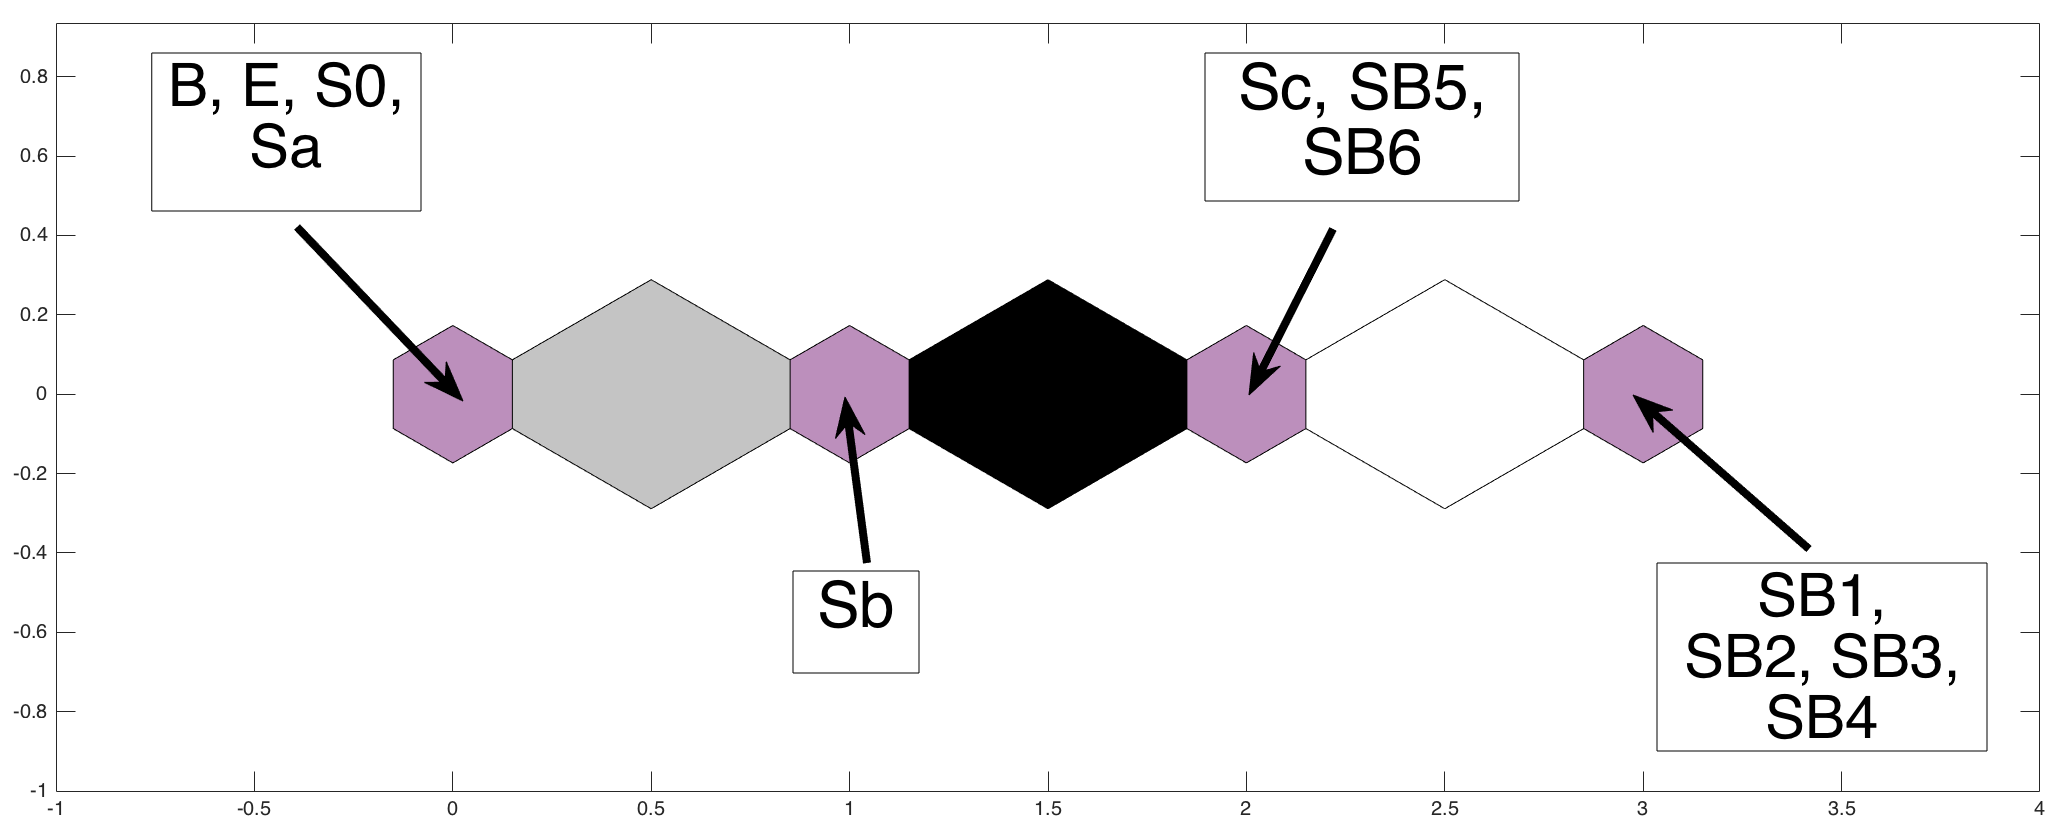
\includegraphics[width=\textwidth]{../images0.01/1d/apps/dist_1_by_4.png}
            %\caption{$1\times4$ weight map}
             %\label{fig: 1by4T}
        \end{subfigure}
        \hfill
        \begin{subfigure}[b]{0.5\textwidth}
             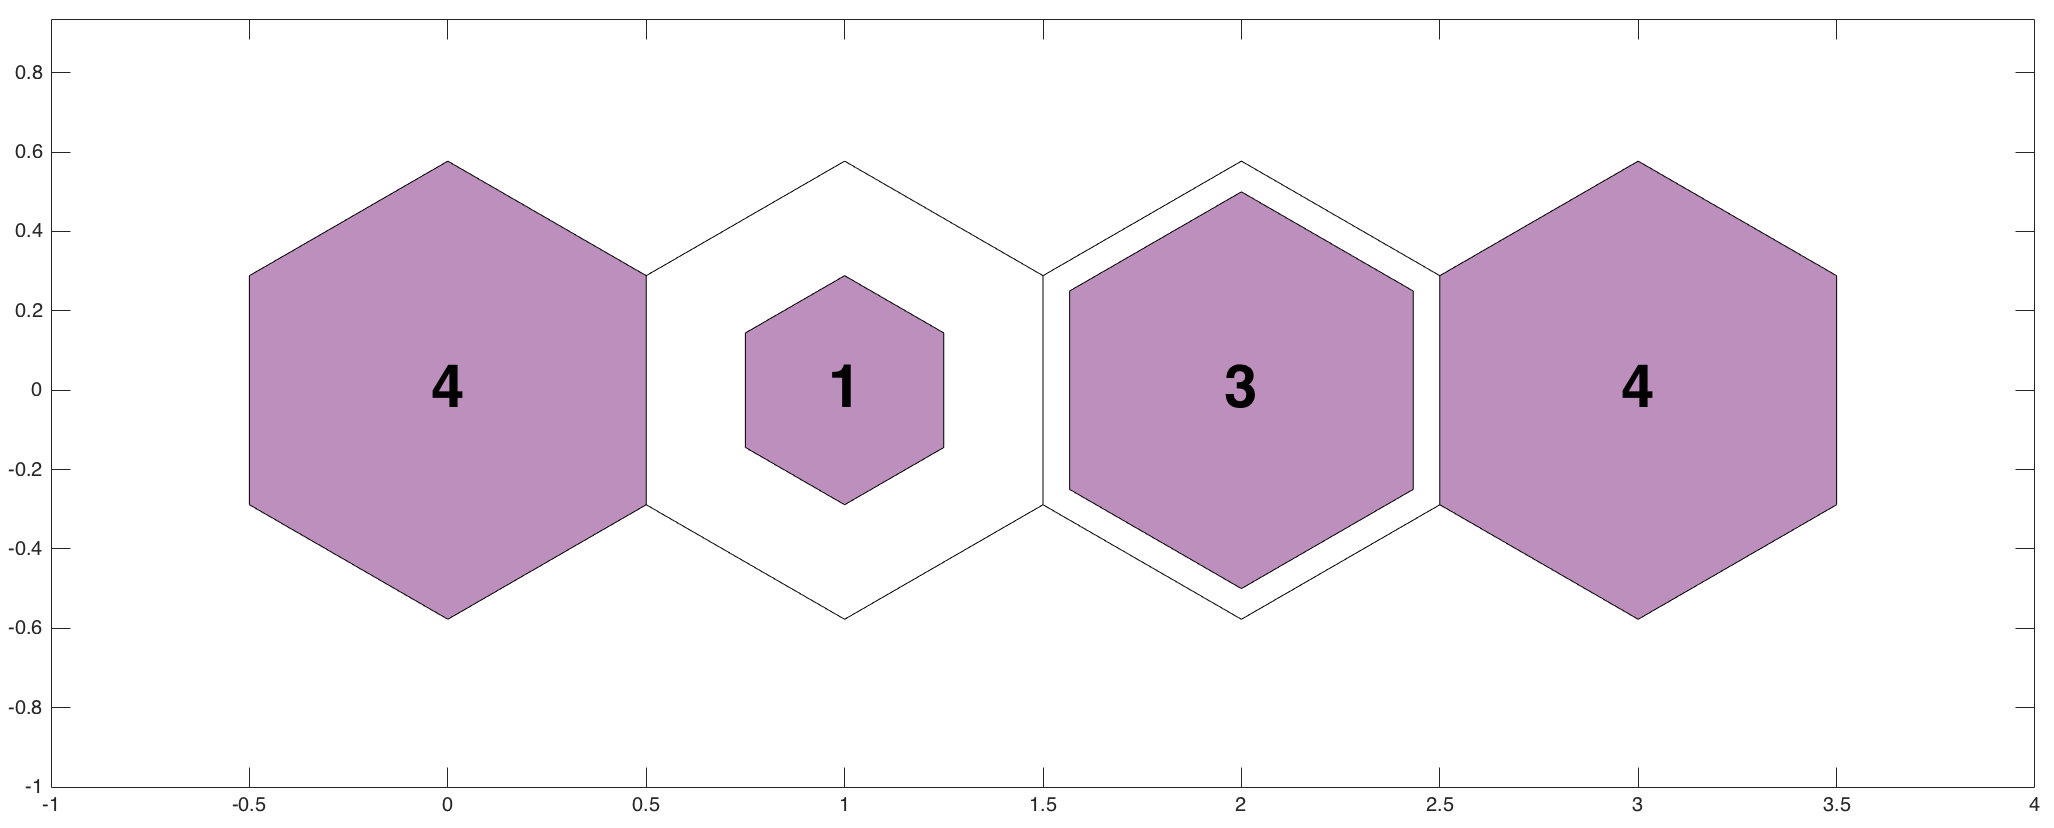
\includegraphics[width=\textwidth]{../images0.01/1d/apps/hit_t_1_by_4.png}
             %\caption{$1\times4$ hits map}
             %\label{fig: 1by4Thits}
        \end{subfigure}
                \caption{Results of training network in $1\times4$~grid.}
         \label{fig: 1by4T}
    \end{figure}
    
    \begin{figure}
        \begin{subfigure}[b]{0.5\textwidth}
            \centering
            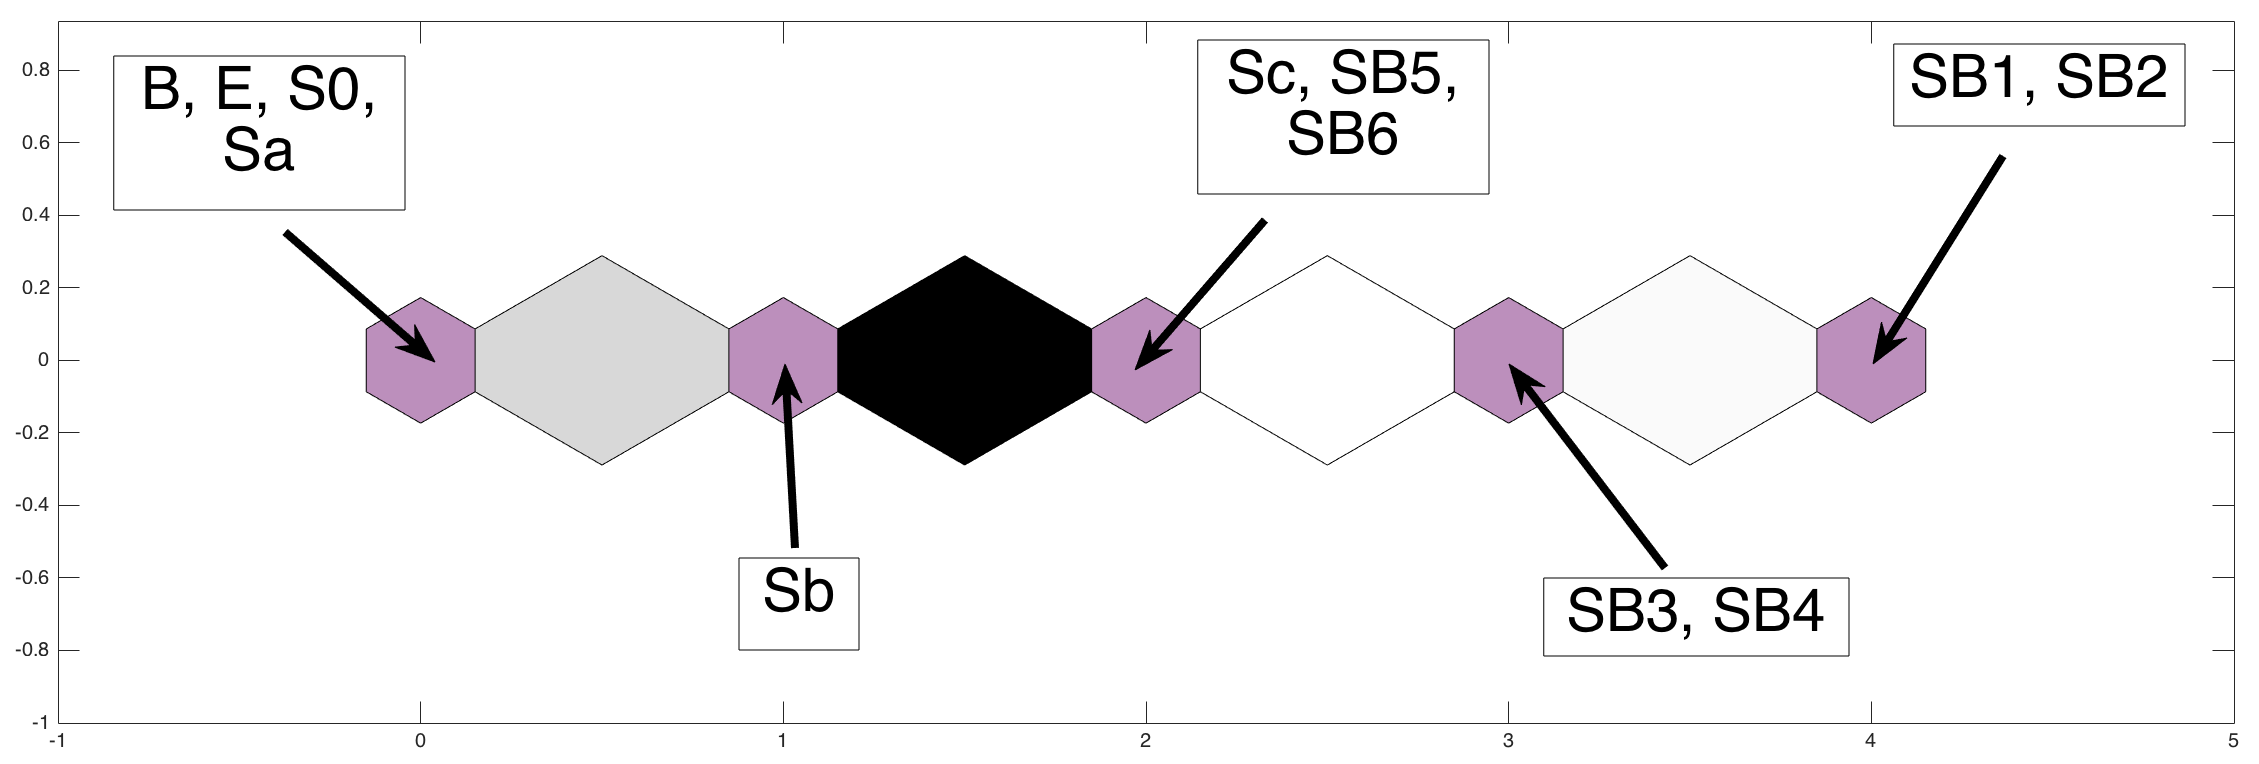
\includegraphics[width=\textwidth]{../images0.01/1d/apps/dist_1_by_5.png}
            %\caption{$1\times5$ weight map}
             %\label{fig: 1by5T}
        \end{subfigure}
        \hfill
        \begin{subfigure}[b]{0.5\textwidth}
             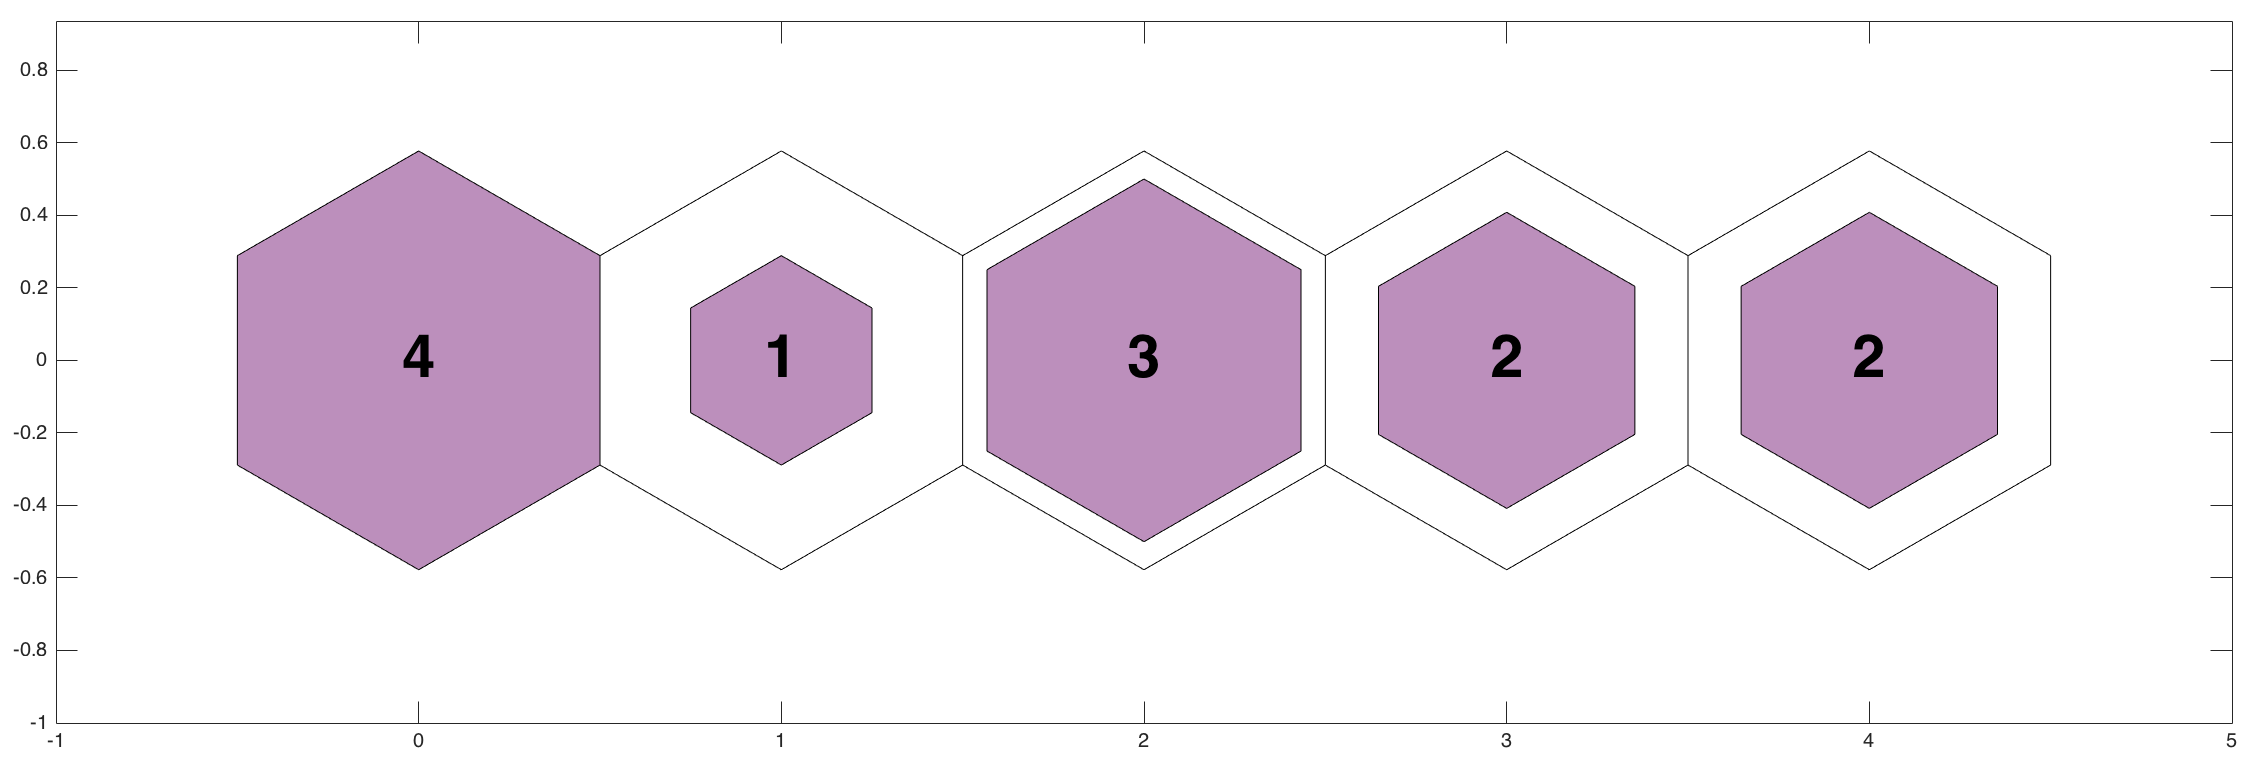
\includegraphics[width=\textwidth]{../images0.01/1d/apps/hit_t_1_by_5.png}
             %\caption{$1\times5$ hits map}
             %\label{fig: 1by5Thits}
        \end{subfigure}
                \caption{Results of training network in $1\times5$~grid.}
         \label{fig: 1by5T}
    \end{figure}
    
    \begin{figure}
        \begin{subfigure}[b]{0.5\textwidth}
            \centering
            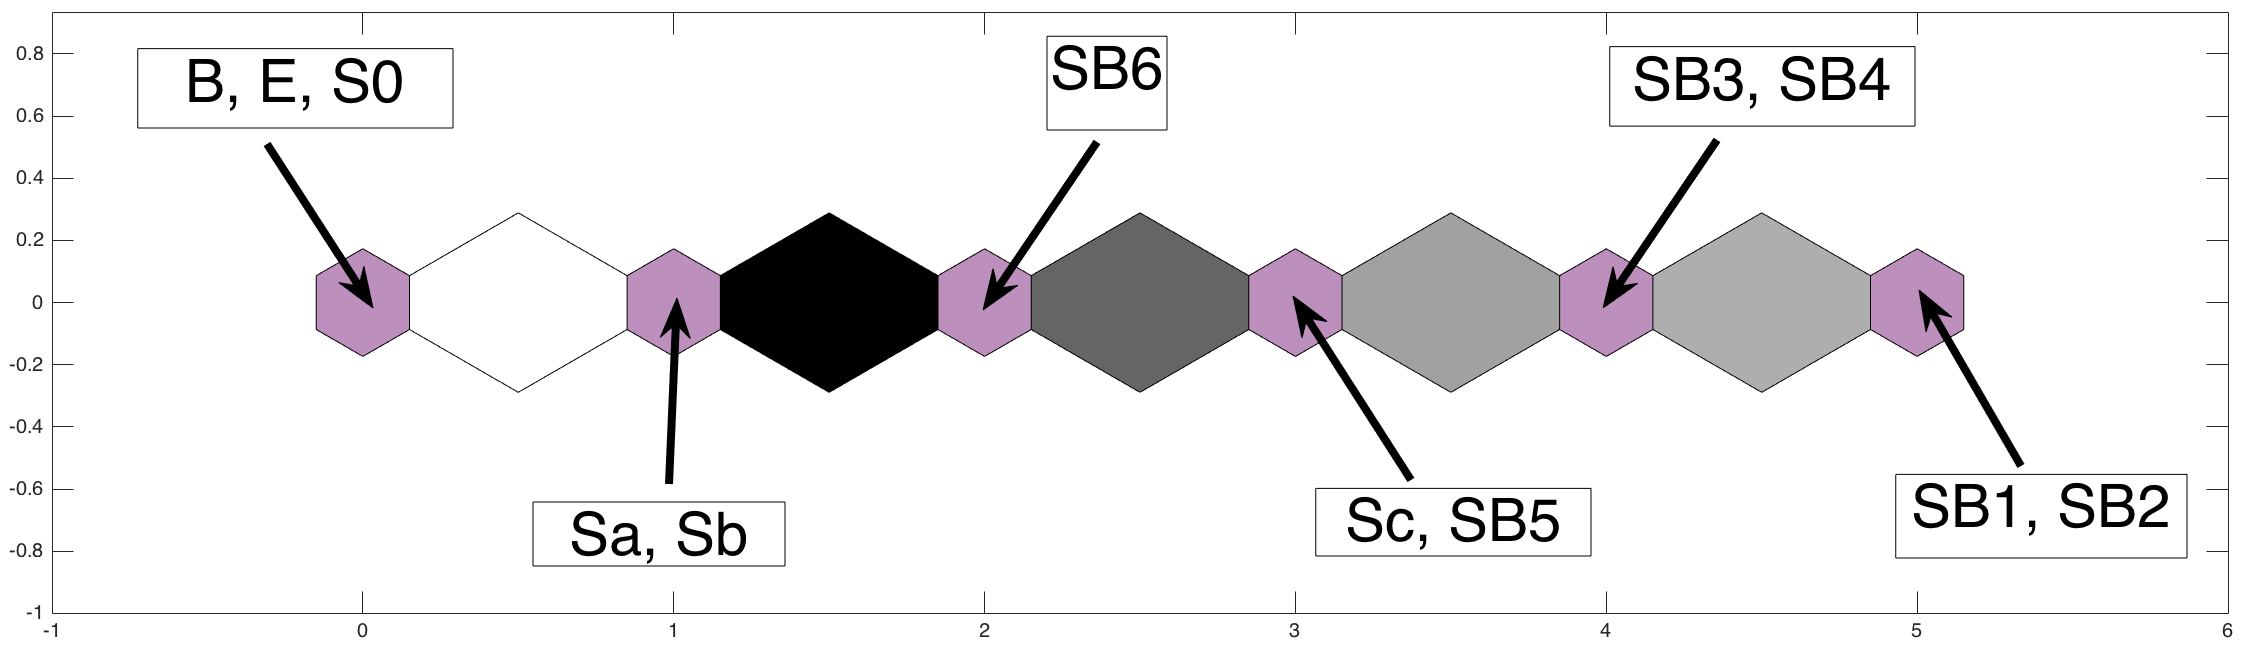
\includegraphics[width=\textwidth]{../images0.01/1d/apps/dist_1_by_6.png}
            %\caption{$1\times6$ weight map}
             %\label{fig: 1by6T}
        \end{subfigure}
        \hfill
        \begin{subfigure}[b]{0.5\textwidth}
             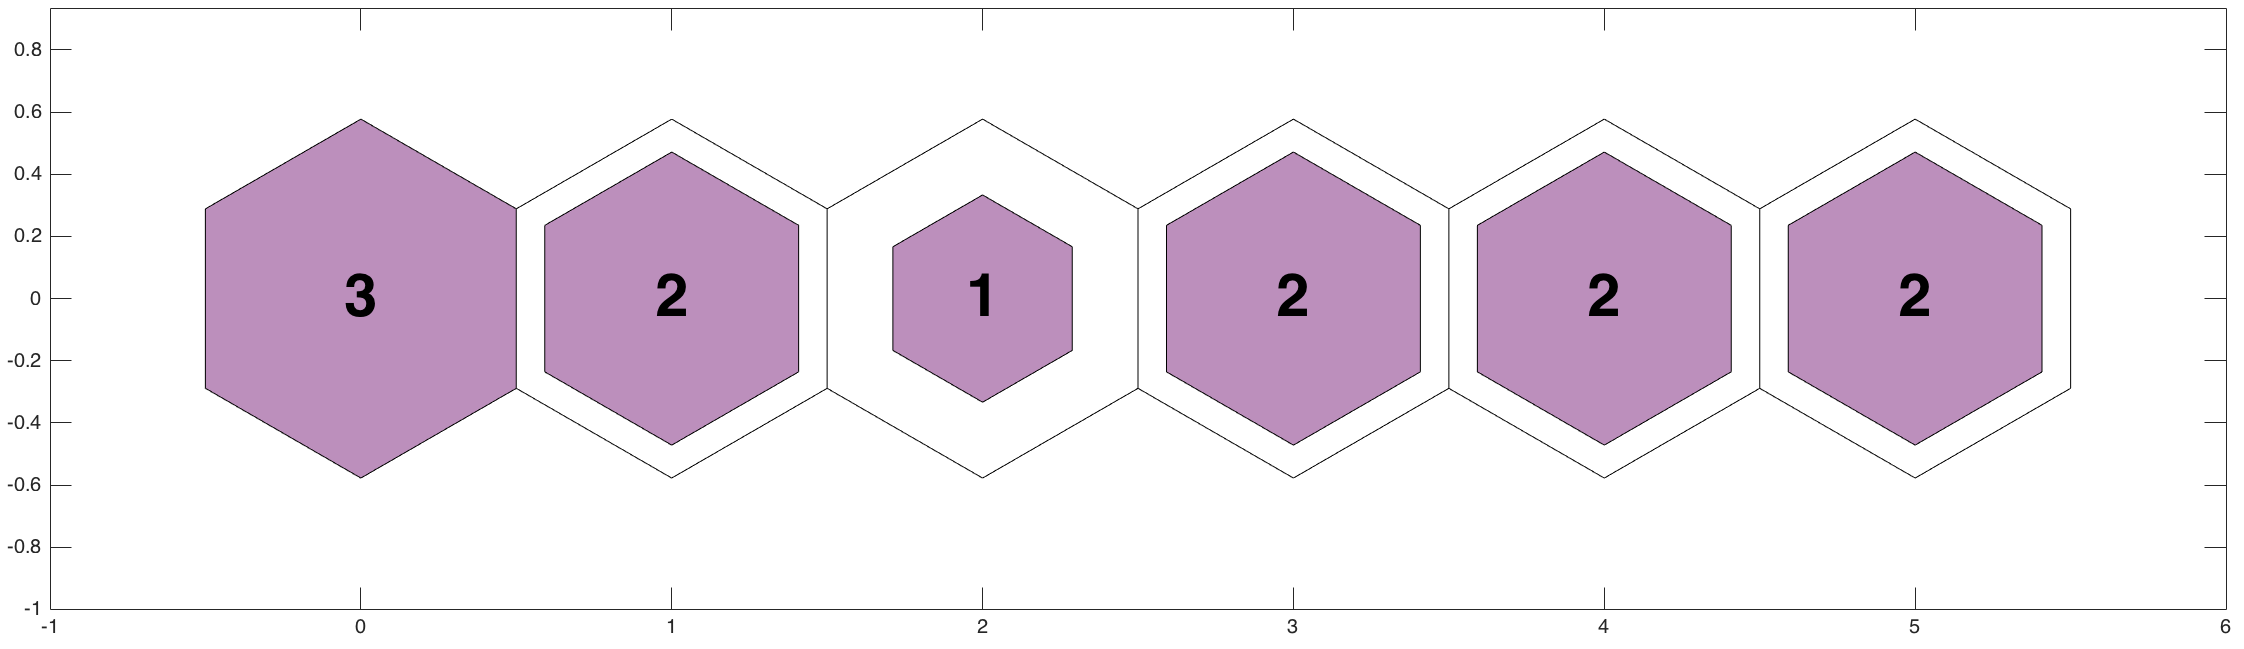
\includegraphics[width=\textwidth]{../images0.01/1d/apps/hit_t_1_by_6.png}
             %\caption{$1\times6$ hits map}
             %\label{fig: 1by6Thits}
        \end{subfigure}
                \caption{Results of training network in $1\times6$~grid.}
         \label{fig: 1by6T}
    \end{figure}
    
    \begin{figure}
        \begin{subfigure}[b]{0.5\textwidth}
            \centering
            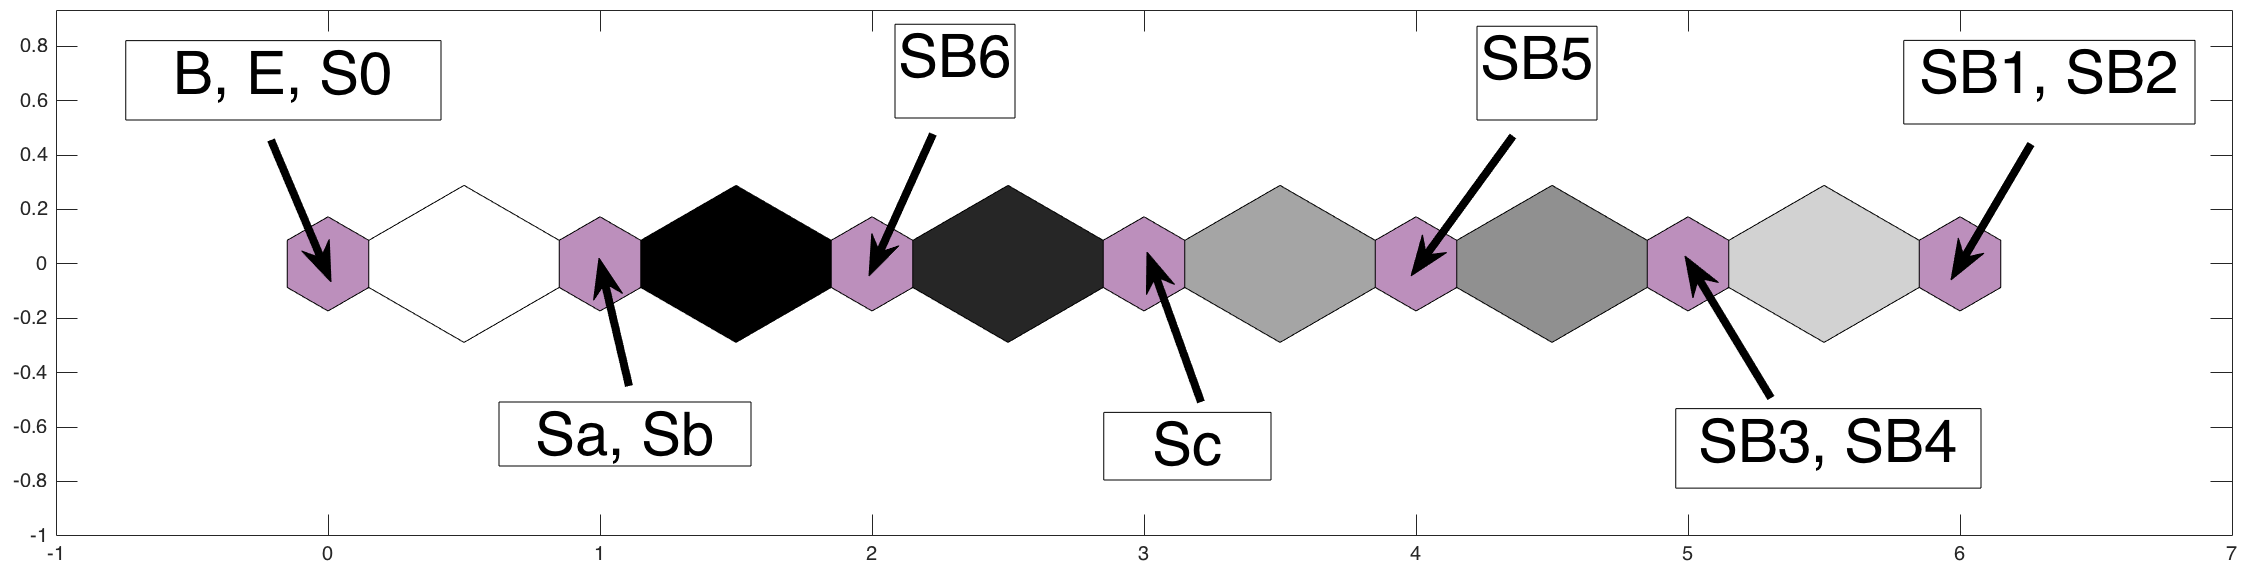
\includegraphics[width=\textwidth]{../images0.01/1d/apps/dist_1_by_7.png}
            %\caption{$1\times7$ weight map}
             %\label{fig: 1by7T}
        \end{subfigure}
        \hfill
        \begin{subfigure}[b]{0.5\textwidth}
             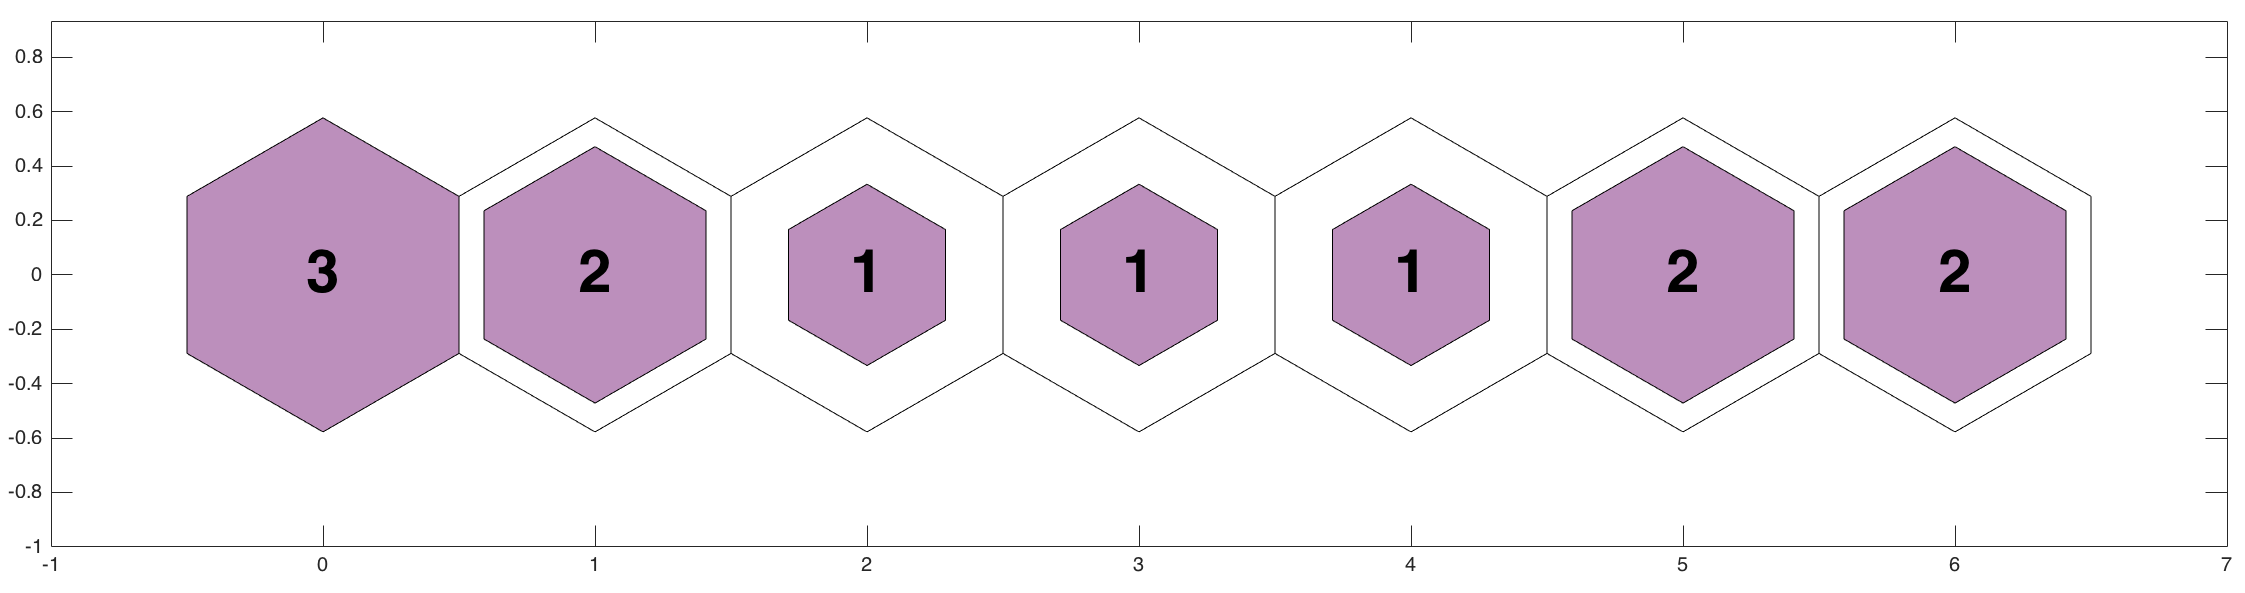
\includegraphics[width=\textwidth]{../images0.01/1d/apps/hit_t_1_by_7.png}
             %\caption{$1\times7$ hits map}
             %\label{fig: 1by7Thits}
        \end{subfigure}
                \caption{Results of training network in $1\times7$~grid.}
         \label{fig: 1by7T}
    \end{figure}
    
    \begin{figure}
        \begin{subfigure}[b]{0.5\textwidth}
            \centering
            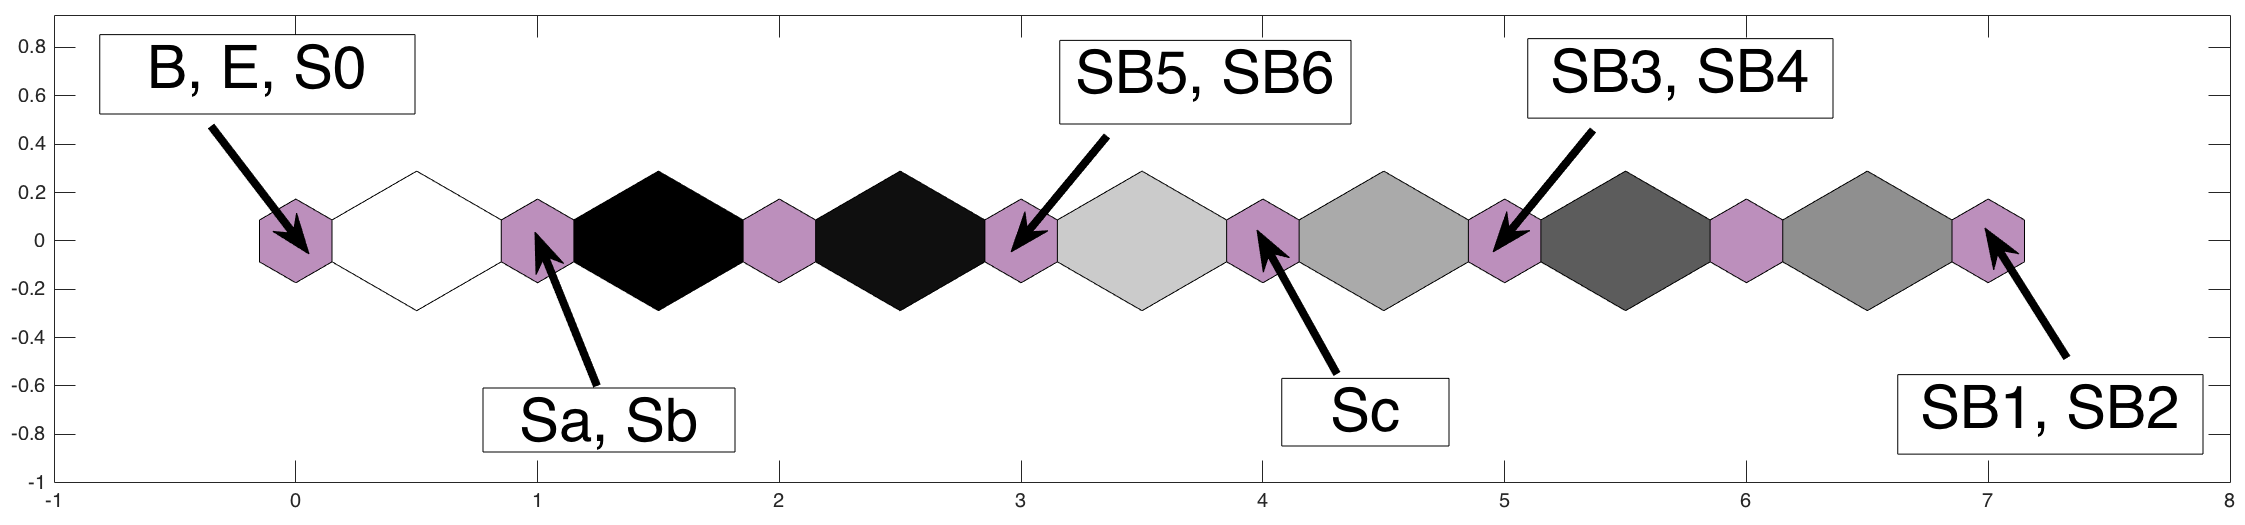
\includegraphics[width=\textwidth]{../images0.01/1d/apps/dist_1_by_8.png}
            %\caption{$1\times8$ weight map}
             %\label{fig: 1by8T}
        \end{subfigure}
        \hfill
        \begin{subfigure}[b]{0.5\textwidth}
             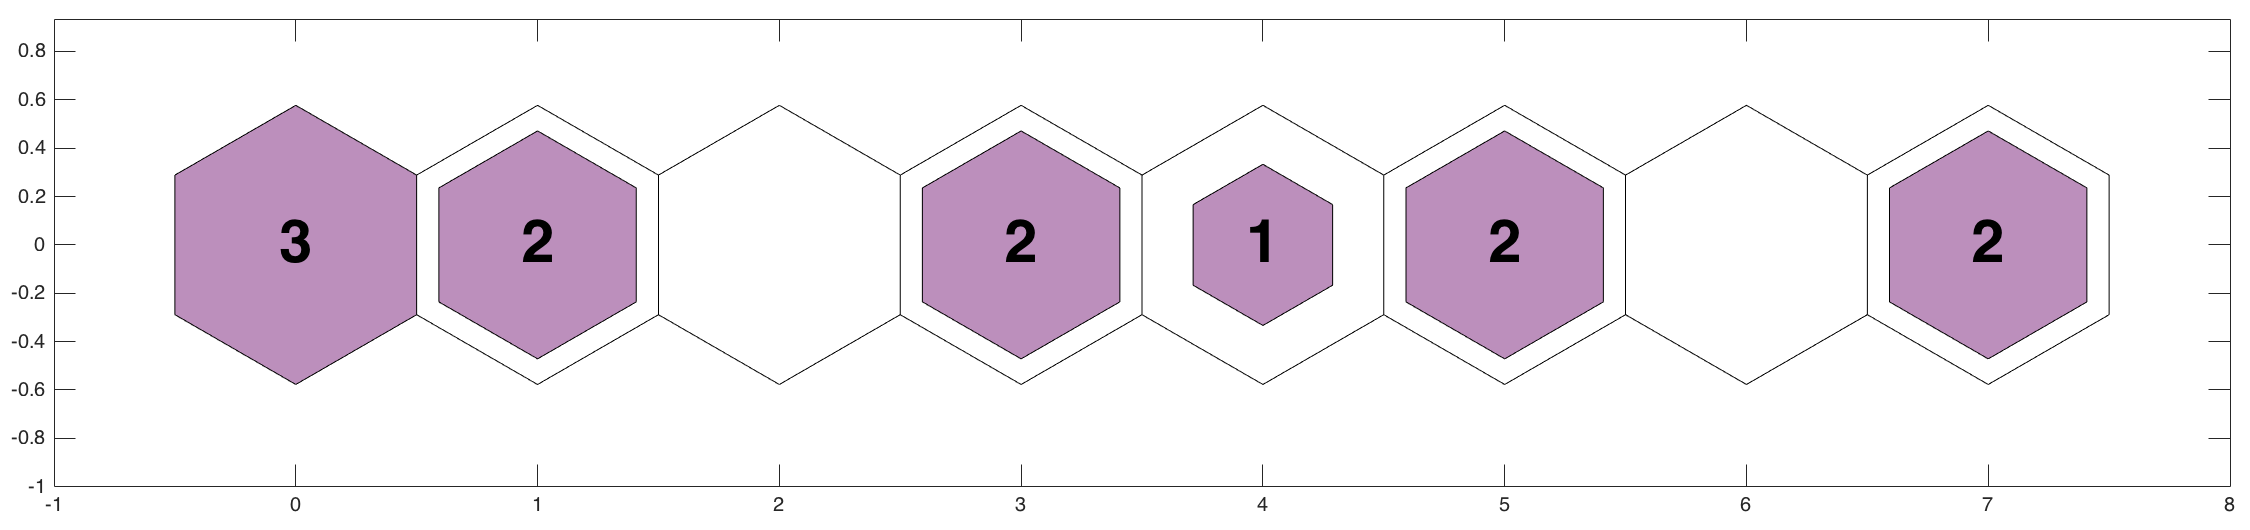
\includegraphics[width=\textwidth]{../images0.01/1d/apps/hit_t_1_by_8.png}
             %\caption{$1\times8$ hits map}
             %\label{fig: 1by8Thits}
        \end{subfigure}
                \caption{Results of training network in $1\times8$~grid.}
         \label{fig: 1by8T}
    \end{figure}
    
    \begin{figure}
        \begin{subfigure}[b]{0.5\textwidth}
            \centering
            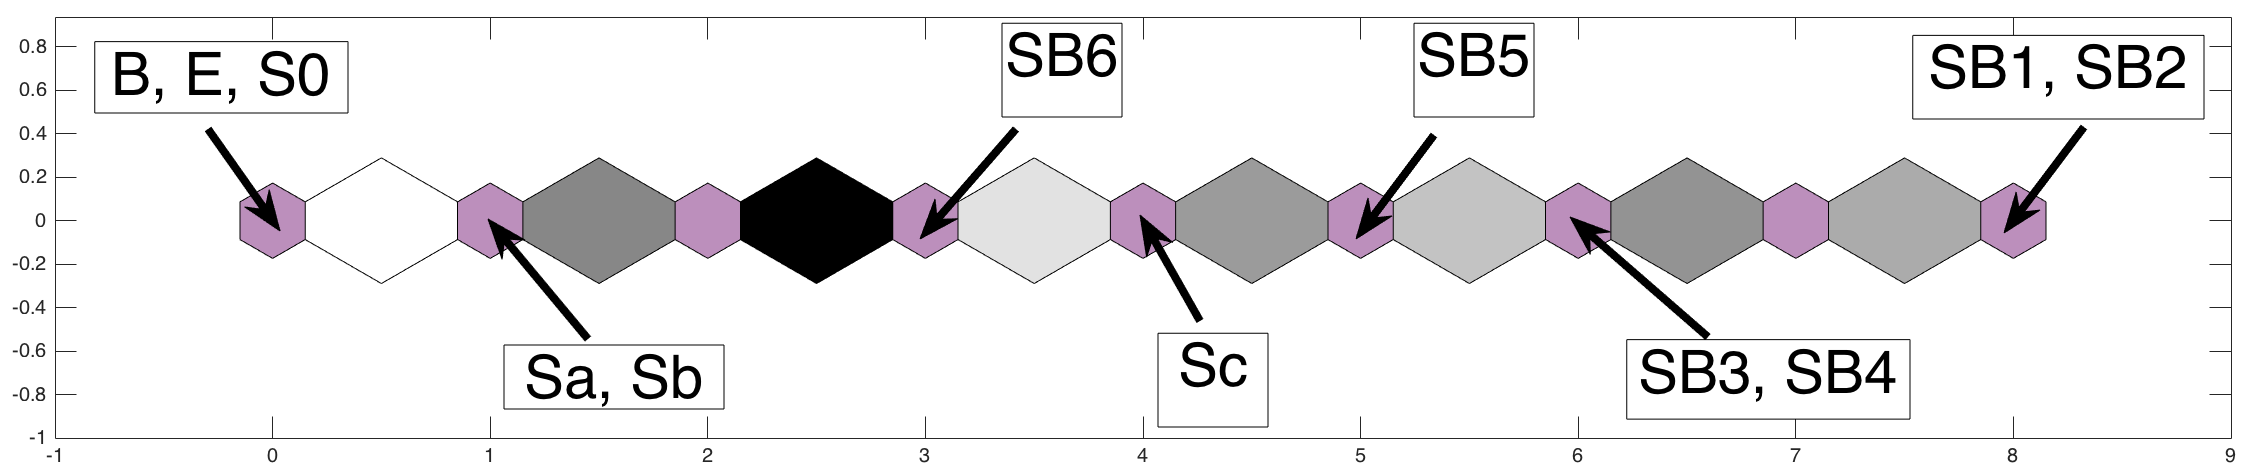
\includegraphics[width=\textwidth]{../images0.01/1d/apps/dist_1_by_9.png}
            %\caption{$1\times9$ weight map}
             %\label{fig: 1by9T}
        \end{subfigure}
        \hfill
        \begin{subfigure}[b]{0.5\textwidth}
             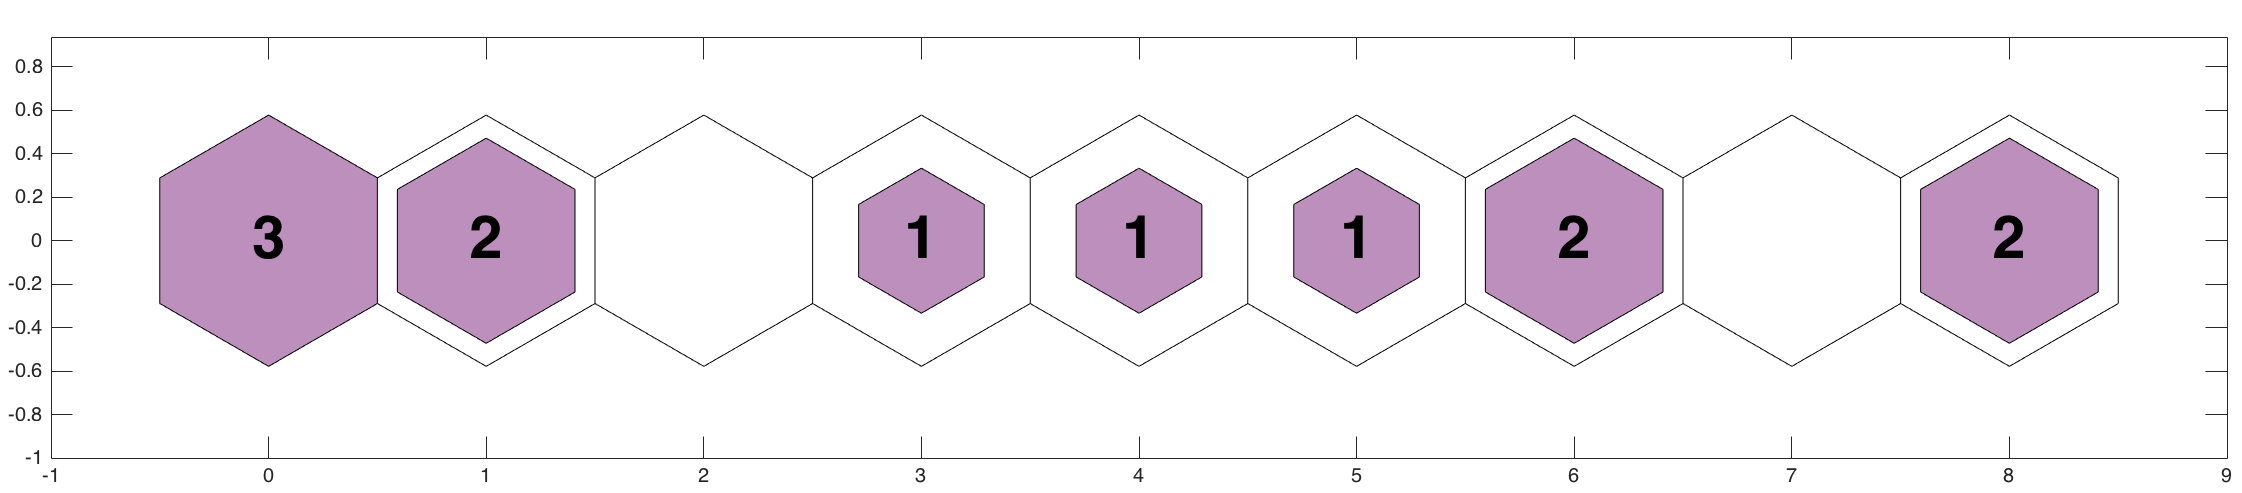
\includegraphics[width=\textwidth]{../images0.01/1d/apps/hit_t_1_by_9.png}
             %\caption{$1\times9$ hits map}
             %\label{fig: 1by9Thits}
        \end{subfigure}
                \caption{Results of training network in $1\times9$~grid.}
         \label{fig: 1by9T}
    \end{figure}

    \begin{figure}
        \begin{subfigure}[b]{0.5\textwidth}
            \centering
            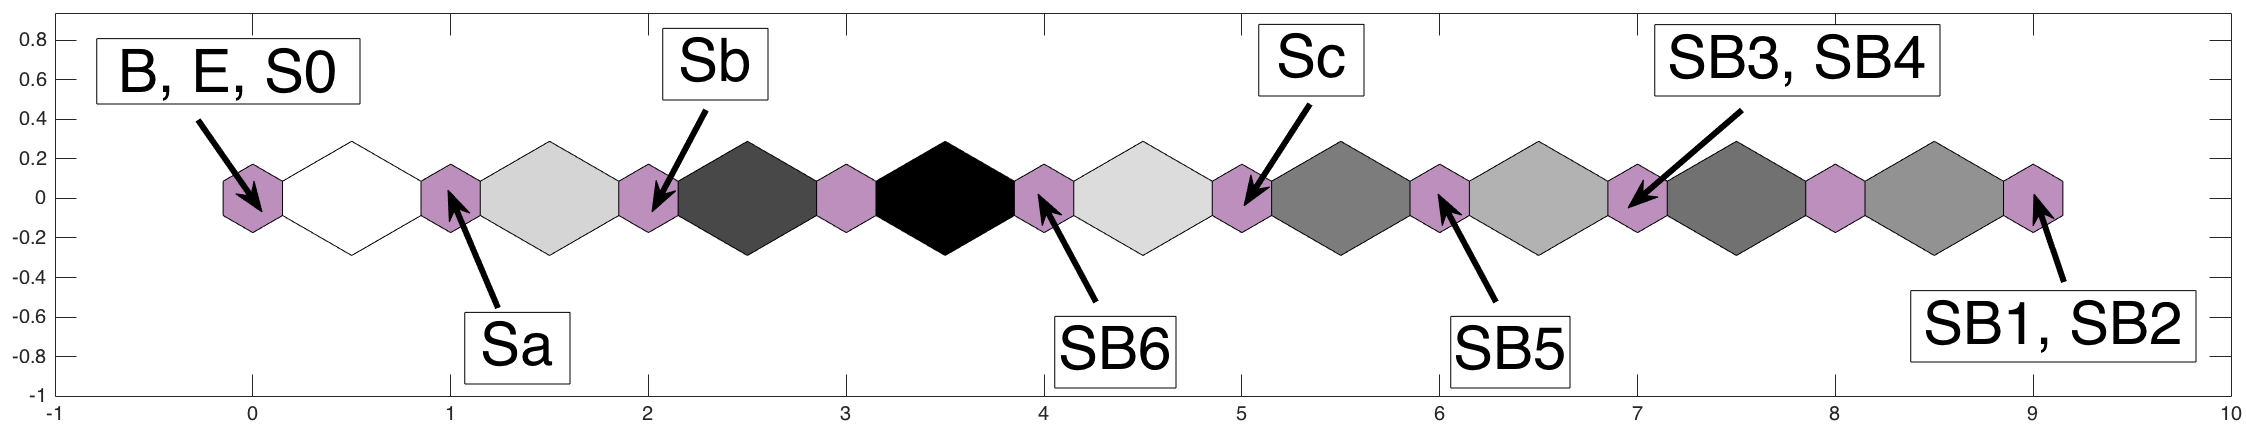
\includegraphics[width=\textwidth,height=2.5cm]{../images0.01/1d/apps/dist_1_by_10.png}
            %\caption{$1\times10$ weight map}
             %\label{fig: 1by10T}
        \end{subfigure}
        \hfill
        \begin{subfigure}[b]{0.5\textwidth}
             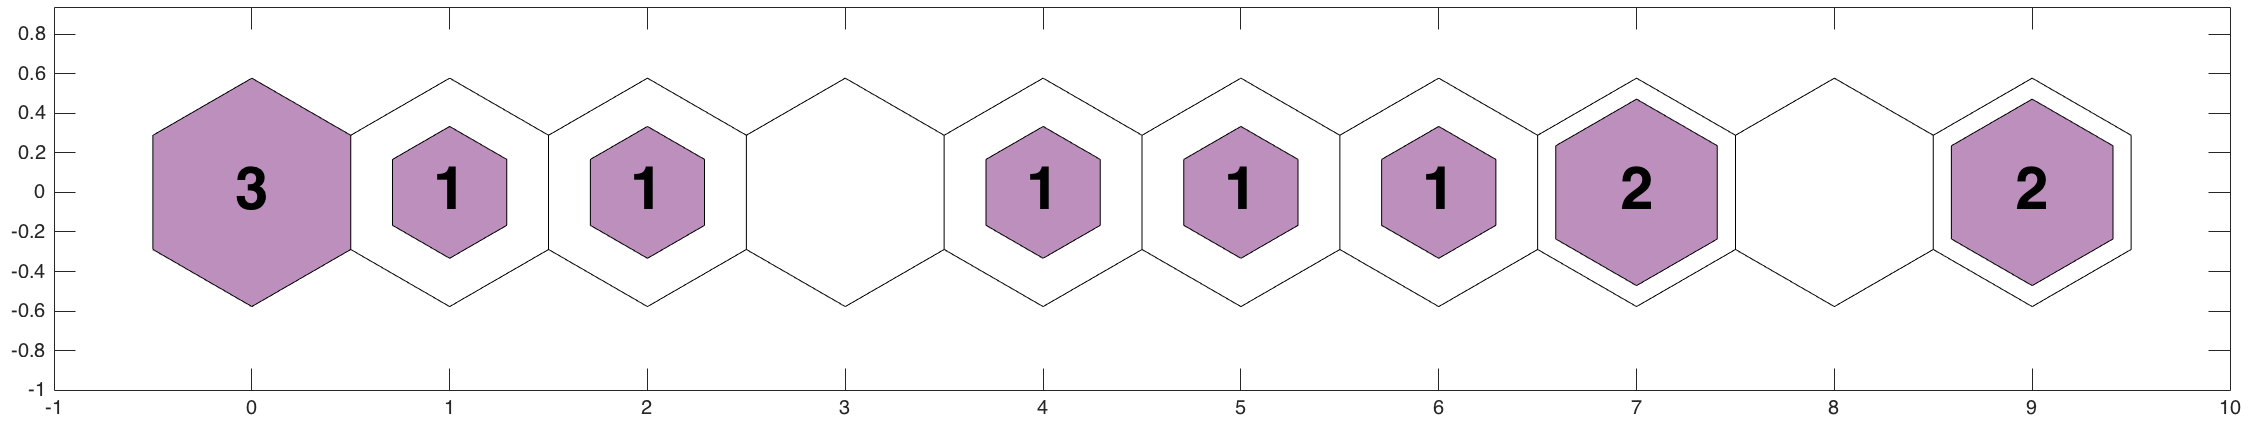
\includegraphics[width=\textwidth,height=2.5cm]{../images0.01/1d/apps/hit_t_1_by_10.png}
             %\caption{$1\times10$ hits map}
             %\label{fig: 1by10Thits}
        \end{subfigure}
                \caption{Results of training network in $1\times10$~grid.}
         \label{fig: 1by10T}
    \end{figure}

    \begin{figure}
        \begin{subfigure}[b]{0.5\textwidth}
            \centering
            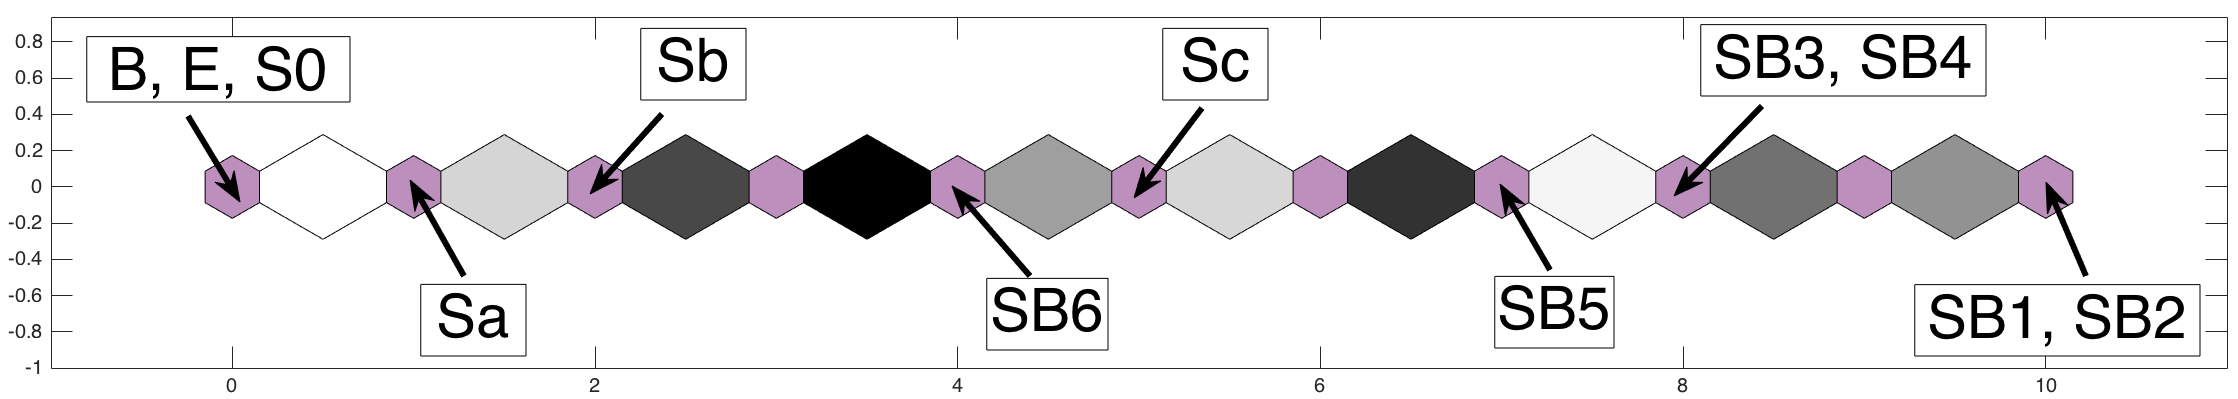
\includegraphics[width=\textwidth,height=2.5cm]{../images0.01/1d/apps/dist_1_by_11.png}
            %\caption{$1\times11$ weight map}
             %\label{fig: 1by11T}
        \end{subfigure}
        \hfill
        \begin{subfigure}[b]{0.5\textwidth}
             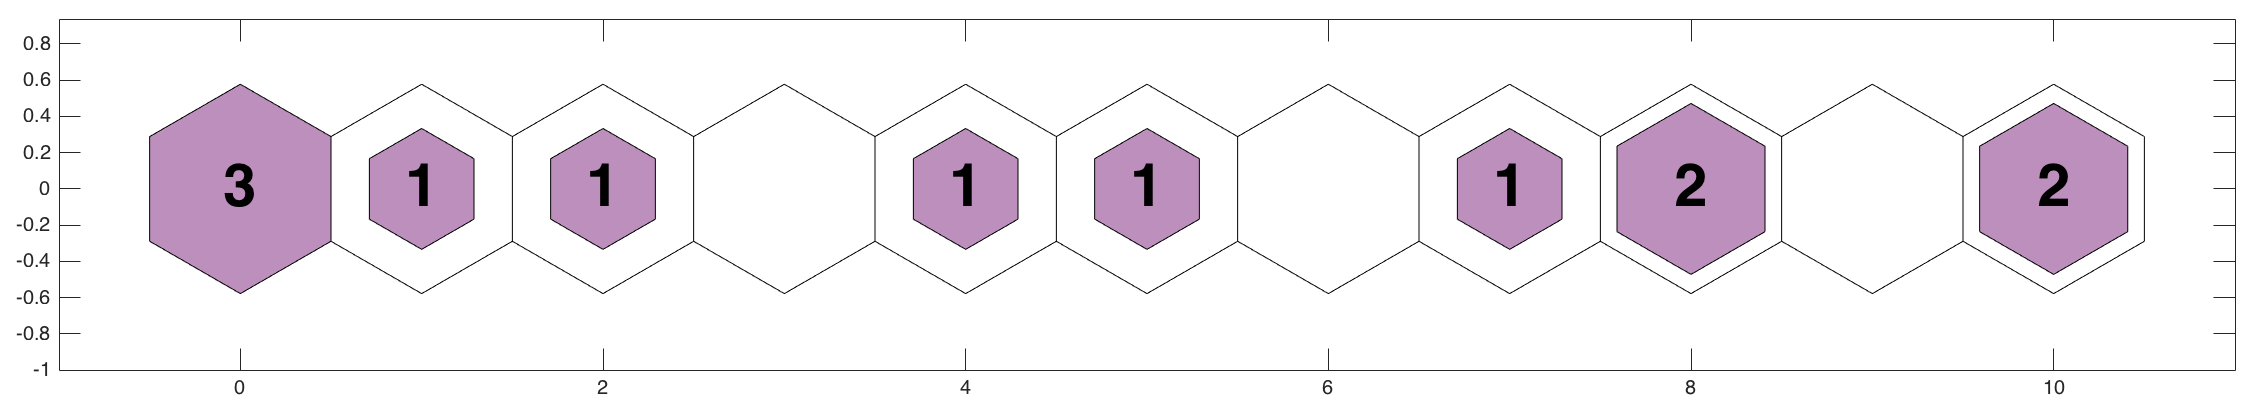
\includegraphics[width=\textwidth,height=2.5cm]{../images0.01/1d/apps/hit_t_1_by_11.png}
             %\caption{$1\times11$ hits map}
             %\label{fig: 1by11Thits}
        \end{subfigure}
                \caption{Results of training network in $1\times11$~grid.}
         \label{fig: 1by11T}
    \end{figure}
    

    \begin{figure}
        \begin{subfigure}[b]{0.5\textwidth}
            \centering
            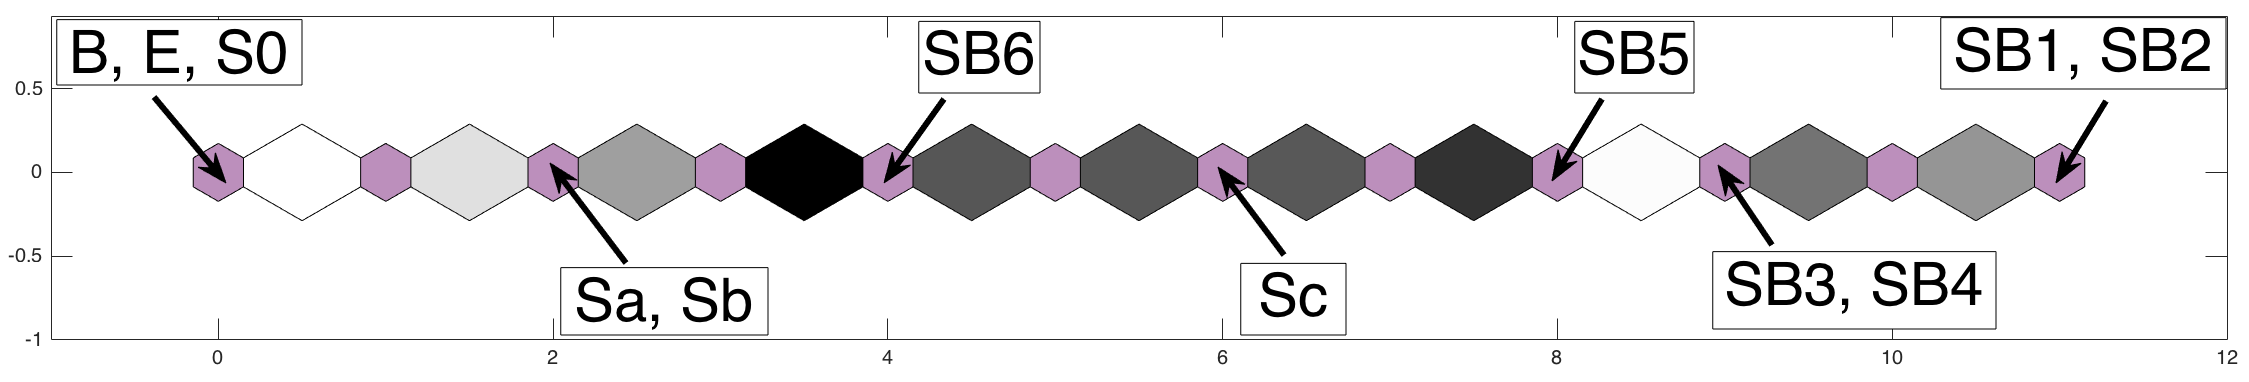
\includegraphics[width=\textwidth,height=2.5cm]{../images0.01/1d/apps/dist_1_by_12.png}
            %\caption{$1\times12$ weight map}
             %\label{fig: 1by12T}
        \end{subfigure}
        \hfill
        \begin{subfigure}[b]{0.5\textwidth}
             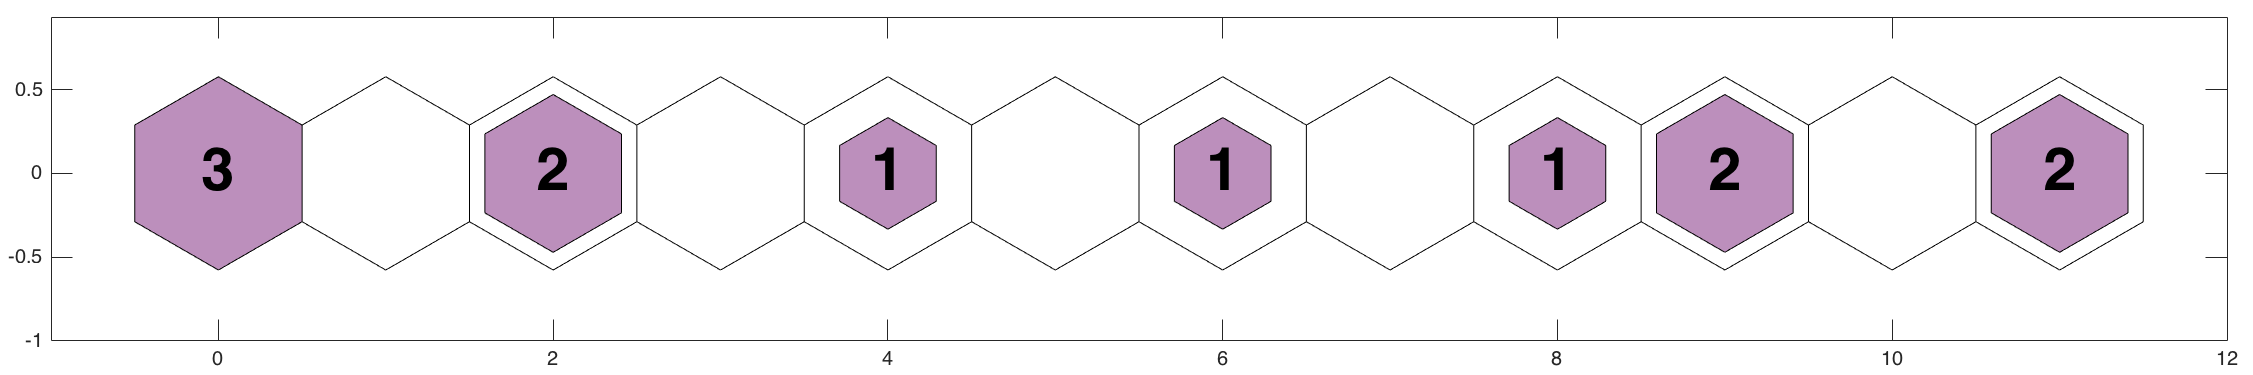
\includegraphics[width=\textwidth,height=2.5cm]{../images0.01/1d/apps/hit_t_1_by_12.png}
             %\caption{$1\times12$ hits map}
             %\label{fig: 1by12Thits}
        \end{subfigure}
                \caption{Results of training network in $1\times12$~grid.}
         \label{fig: 1by12T}
    \end{figure}

    \begin{figure}
        \begin{subfigure}[b]{0.5\textwidth}
            \centering
            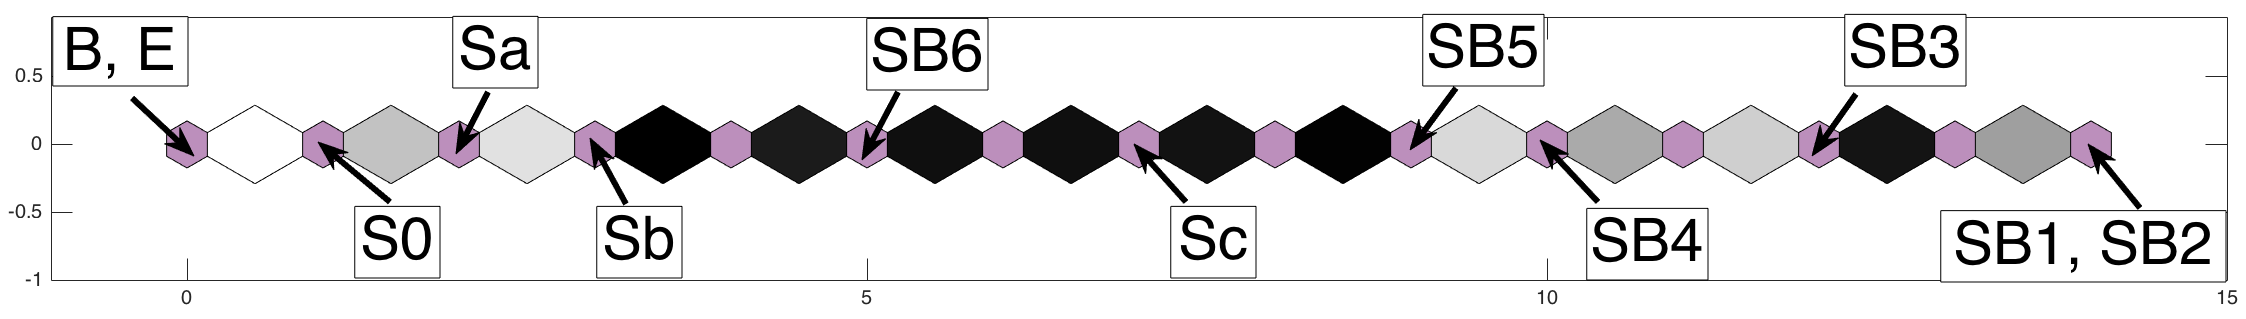
\includegraphics[width=\textwidth,height=2.5cm]{../images0.01/1d/apps/dist_1_by_15.png}
            %\caption{$1\times15$ weight map}
             %\label{fig: 1by15T}
        \end{subfigure}
        \hfill
        \begin{subfigure}[b]{0.5\textwidth}
             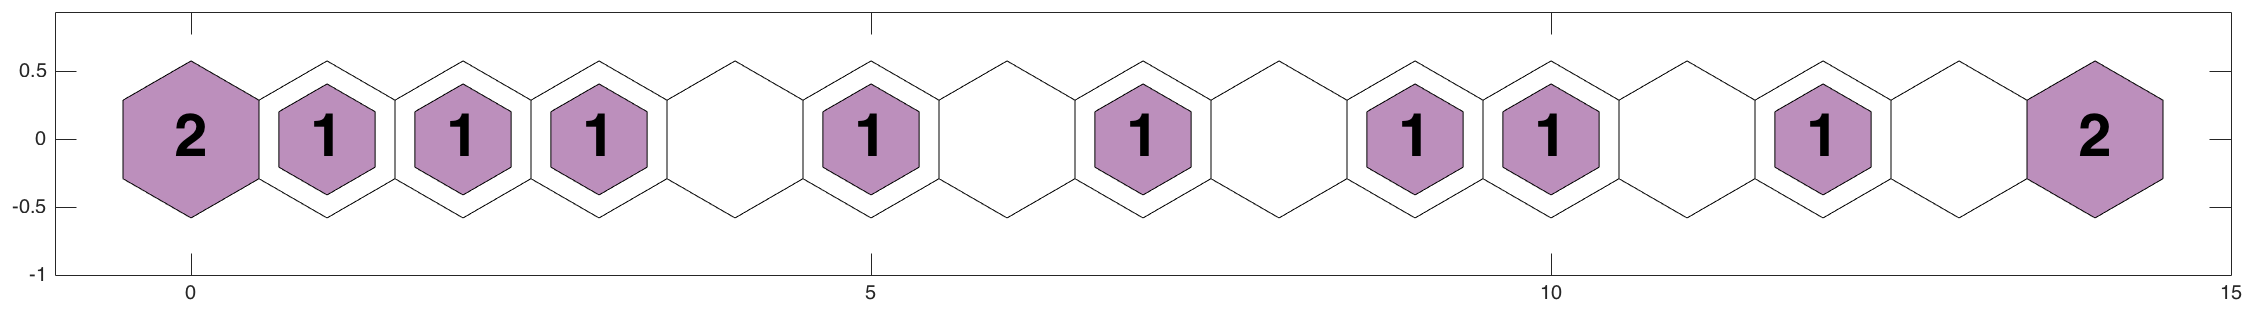
\includegraphics[width=\textwidth,height=2.5cm]{../images0.01/1d/apps/hit_t_1_by_15.png}
             %\caption{$1\times15$ hits map}
             %\label{fig: 1by15Thits}
        \end{subfigure}
                \caption{Results of training network in $1\times15$~grid.}
         \label{fig: 1by15T}
    \end{figure}

    \begin{figure}
        \begin{subfigure}[b]{0.5\textwidth}
            \centering
            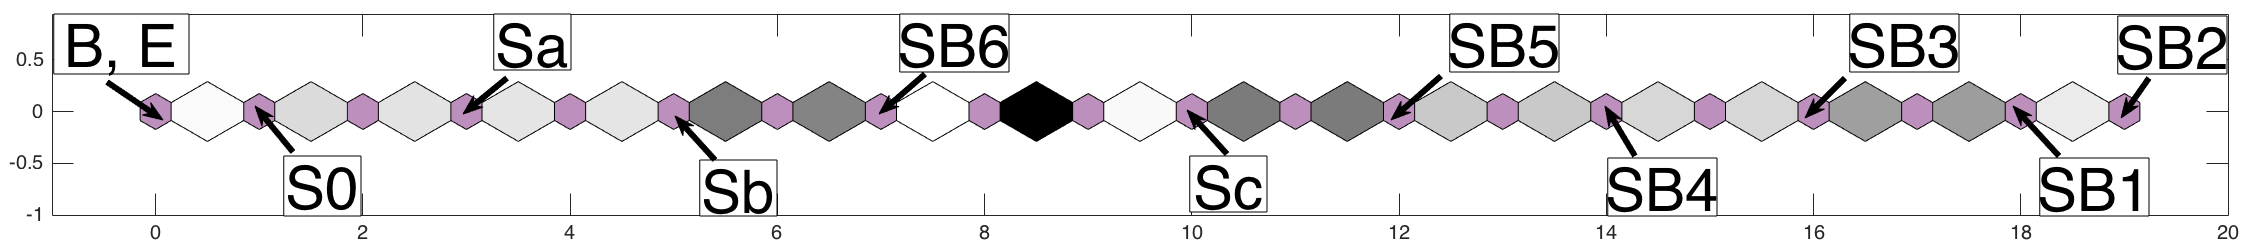
\includegraphics[width=\textwidth,height=2.5cm]{../images0.01/1d/apps/dist_1_by_20.png}
            %\caption{$1\times20$ weight map}
             %\label{fig: 1by20T}
        \end{subfigure}
        \hfill
        \begin{subfigure}[b]{0.5\textwidth}
             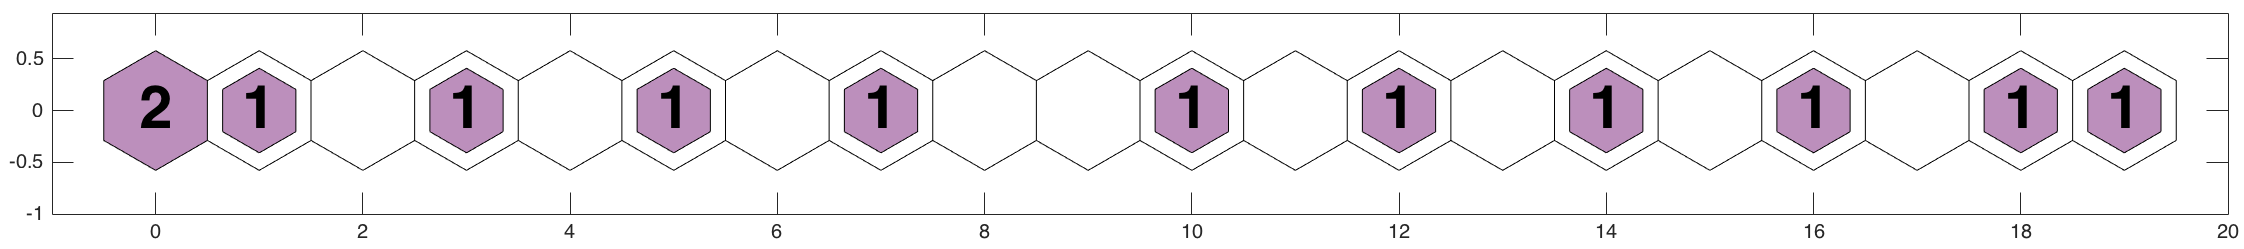
\includegraphics[width=\textwidth,height=2.5cm]{../images0.01/1d/apps/hit_t_1_by_20.png}
             %\caption{$1\times20$ hits map}
             %\label{fig: 1by20Thits}
        \end{subfigure}
                \caption{Results of training network in $1\times20$~grid.}
         \label{fig: 1by20T}
    \end{figure}
    

\newpage

\section{Comparison of the self-organizing maps and K-means methods}
\label{app: high_Z_1d_k-means}


In this section we present the result of applying  K-means clustering method on the the spectra of 142 galaxies from \citetalias{Hossein12}.
K-means clustering, alongside of SOMs are two of main unsupervised methods that are being used in astronomical studies \citep[e.g.][]{DAbrusco12, Aycha16}.
In the K-means methods, the user decides number of cluster, K. 
The algorithm, randomly chooses K random points to be set as a centroid of the clusters.
Then, it finds the data points that are closer to the each assumed centroid and cluster them together.
Mean values of the data points that are assigned to each cluster were calculated and become the new centroid of the cluster. 
The algorithm finds new clusters based on the new centroids and repeats the procedure until it converges. 
We used \textsc{matlab} K-means library to perform the K-means clustering.

For analyzing our data using the spectra of 142 sample galaxies, we set the number of clusters from 2 to 22.
We calculate the median of the spectra in each cluster, and compare the medians with the \citetalias{Kinney96} templates.
To find the best match between the medians and the templates, we measured the spectral angle distance between them as follow:
\begin{equation}
    cos(\theta) = \frac{\sum_{i=1}^{n} s_it_i}{(\sum_{i=1}^{n} s^2_i)^{0.5} (\sum_{i=1}^{n} t^2_i)^{0.5}}
\end{equation}
where $s_i$ and $t_i$ are the ith wavelength of sample and template spectra, respectively. 
$\theta$ is the angle between the spectrum, that the zero value means completely similar and the 180  degree means the completely different spectra. Since $cos(\theta)$, changes between -1 and 1, 1-$cos(\theta)$ would be the easier way to measure and report the distance.
In this case the minimum of 1-$cos(\theta)$ for each set, would be the best match.

% \ref{fig: k-means22} shows the median spectra of the members of the 22 clusters (solid black lines) and the best match from \citetalias{Kinney96} templates (dash-dot red lines).
% As it clears in the figure, although the K-means clustering method separated the spectra of sample galaxies into 22 different groups, only 7 of template spectra matches the best with these 22 groups and the rest are completely ignored. 
% The other problem, is that in this method, in some cases even the most similar template spectra is not a good fit to the median spectra of the clusters.

\begin{figure*}
                \begin{subfigure}[b]{0.49\textwidth}
                    \centering
                  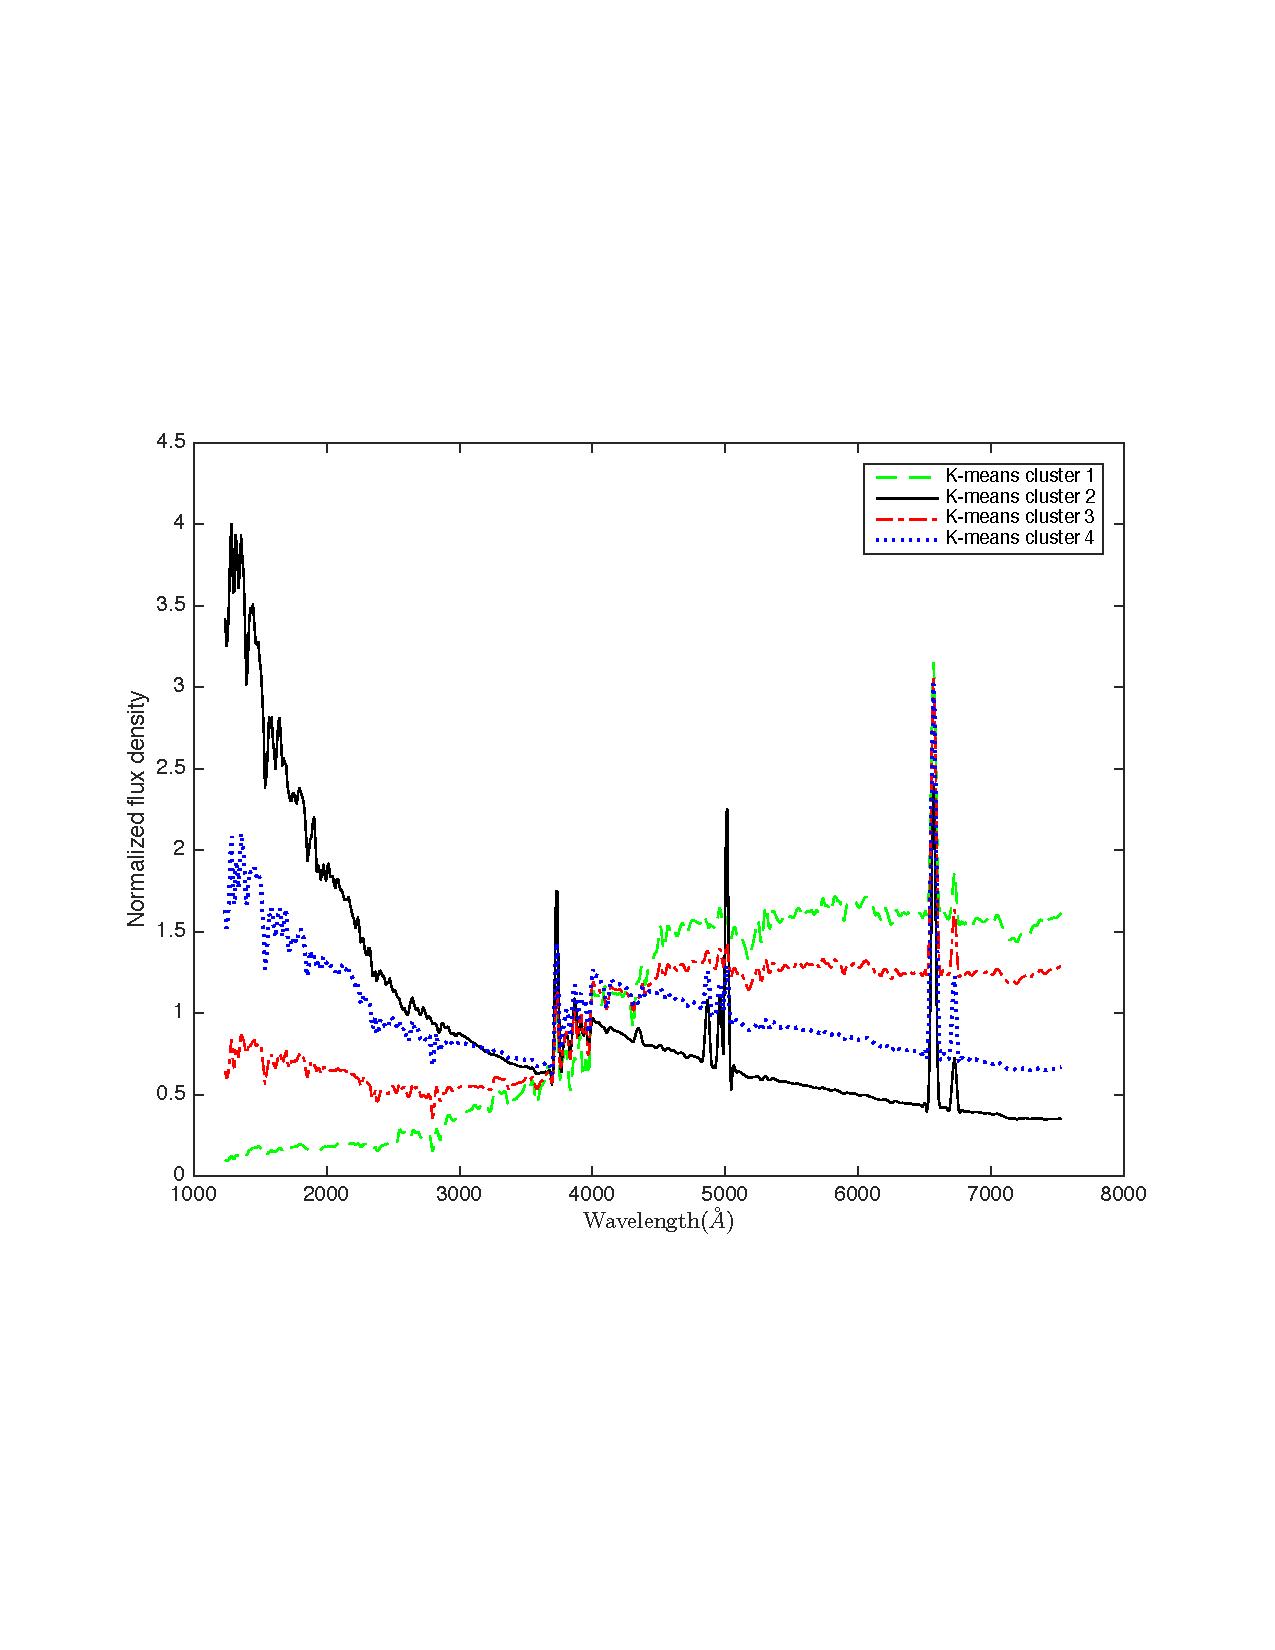
\includegraphics[width=.99\textwidth]{k_means_images/classified_group_in_4cluster_142.pdf}
                \end{subfigure}
                \hfill
                \begin{subfigure}[b]{0.49\textwidth}
                    \centering 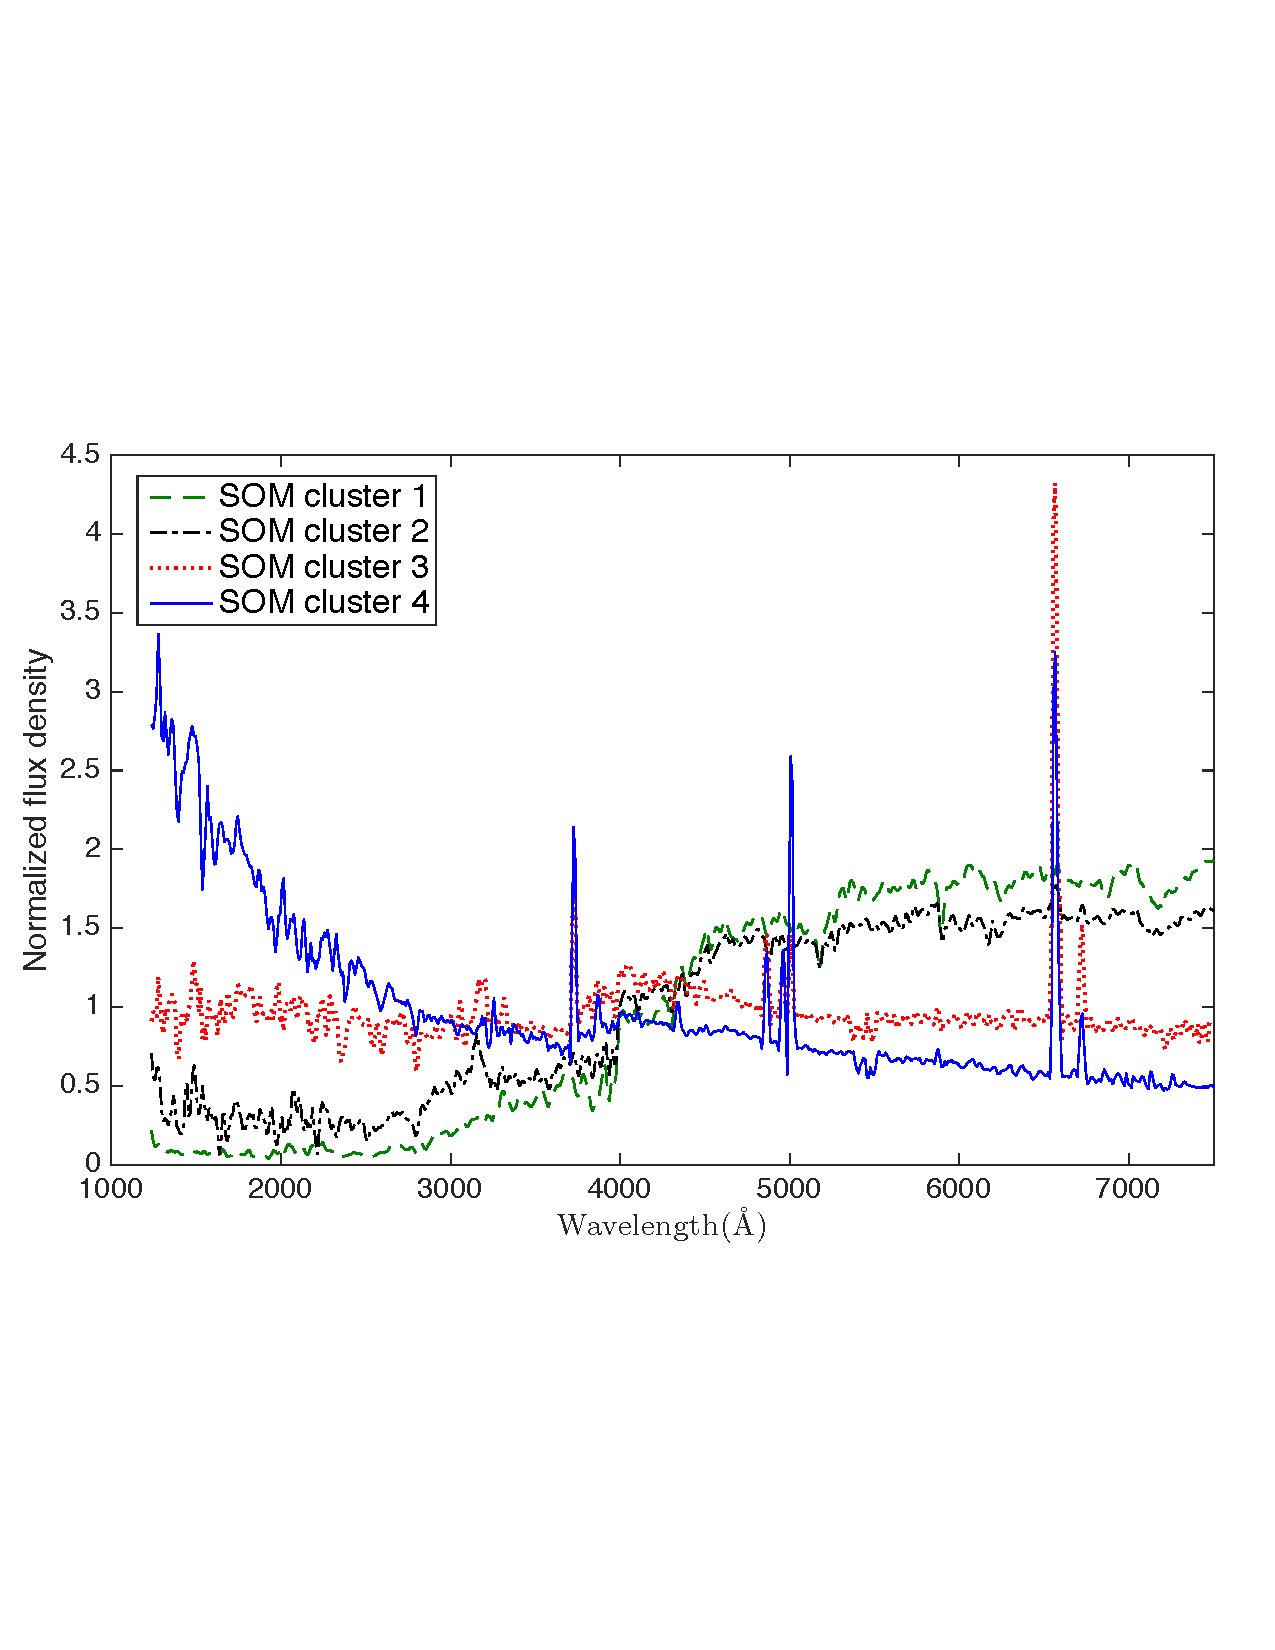
\includegraphics[width=.99\textwidth]{k_means_images/classified_group_in_4cluster_som.pdf}
                \end{subfigure}
                \caption{km}
                 \label{fig: som_k_means_4}
\end{figure*}



\begin{figure}
                \begin{subfigure}[b]{0.49\textwidth}
                    \centering
                  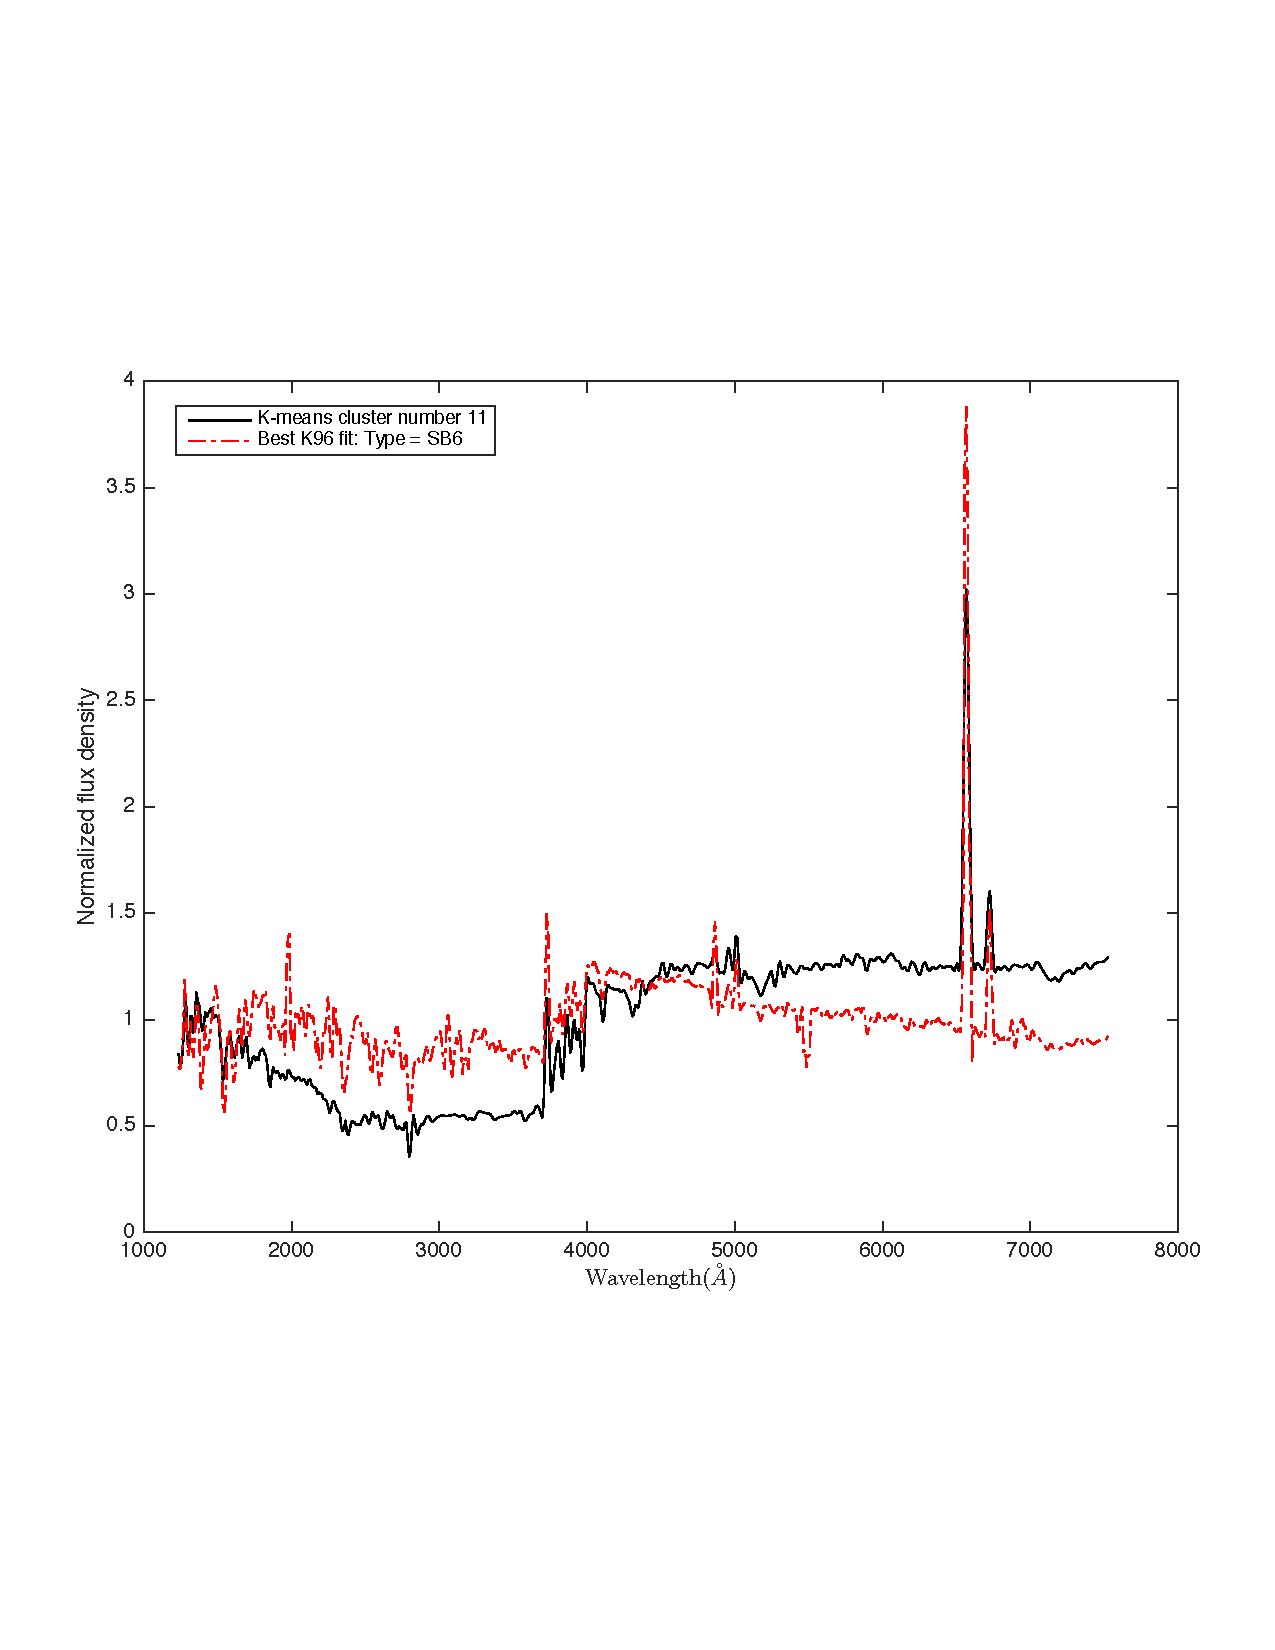
\includegraphics[width=.99\textwidth]{k_means_images/max_cosine2.pdf}
                \end{subfigure}
                \hfill
                \begin{subfigure}[b]{0.49\textwidth}
                    \centering 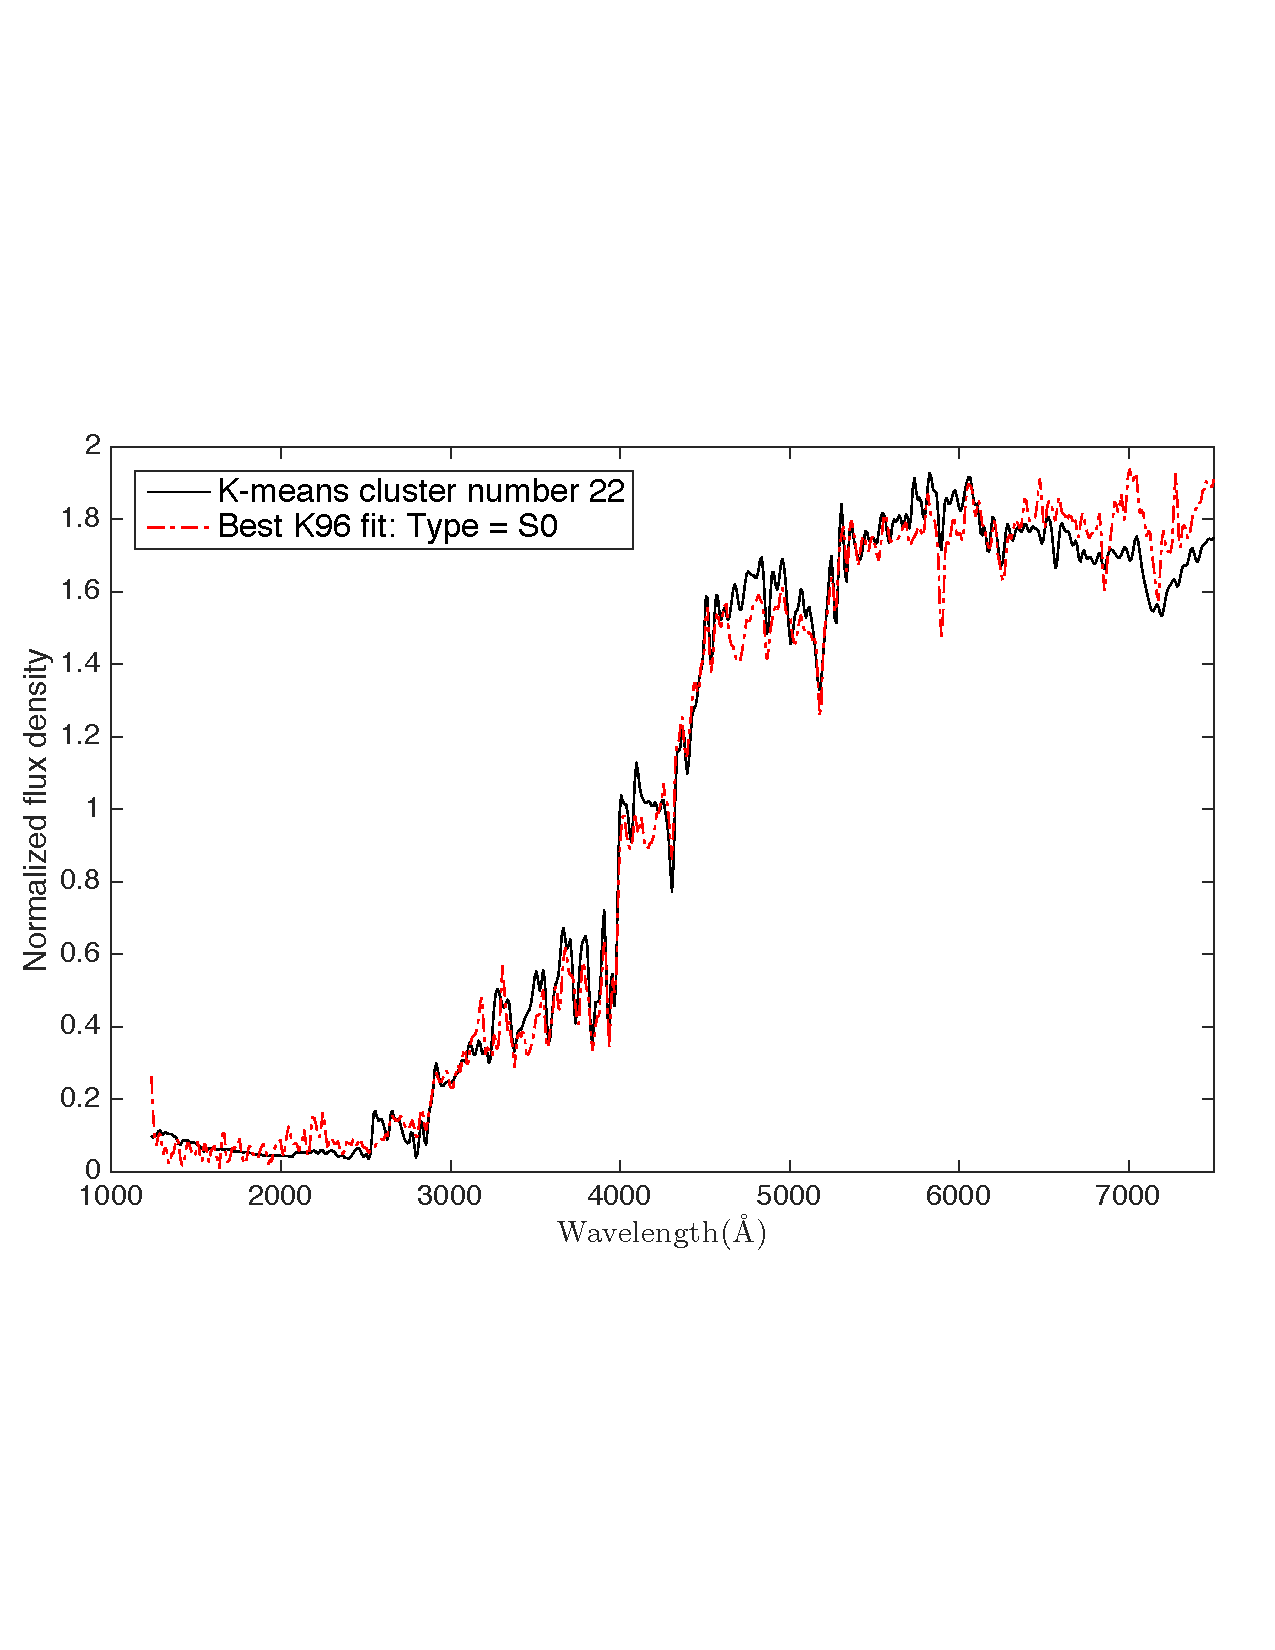
\includegraphics[width=.99\textwidth]{k_means_images/min_cosine2.pdf}
                \end{subfigure}
                \caption{km}
                 \label{fig: k_means_minmax}
\end{figure}



\begin{figure}
                \begin{subfigure}[b]{0.5\textwidth}
                    \centering
                  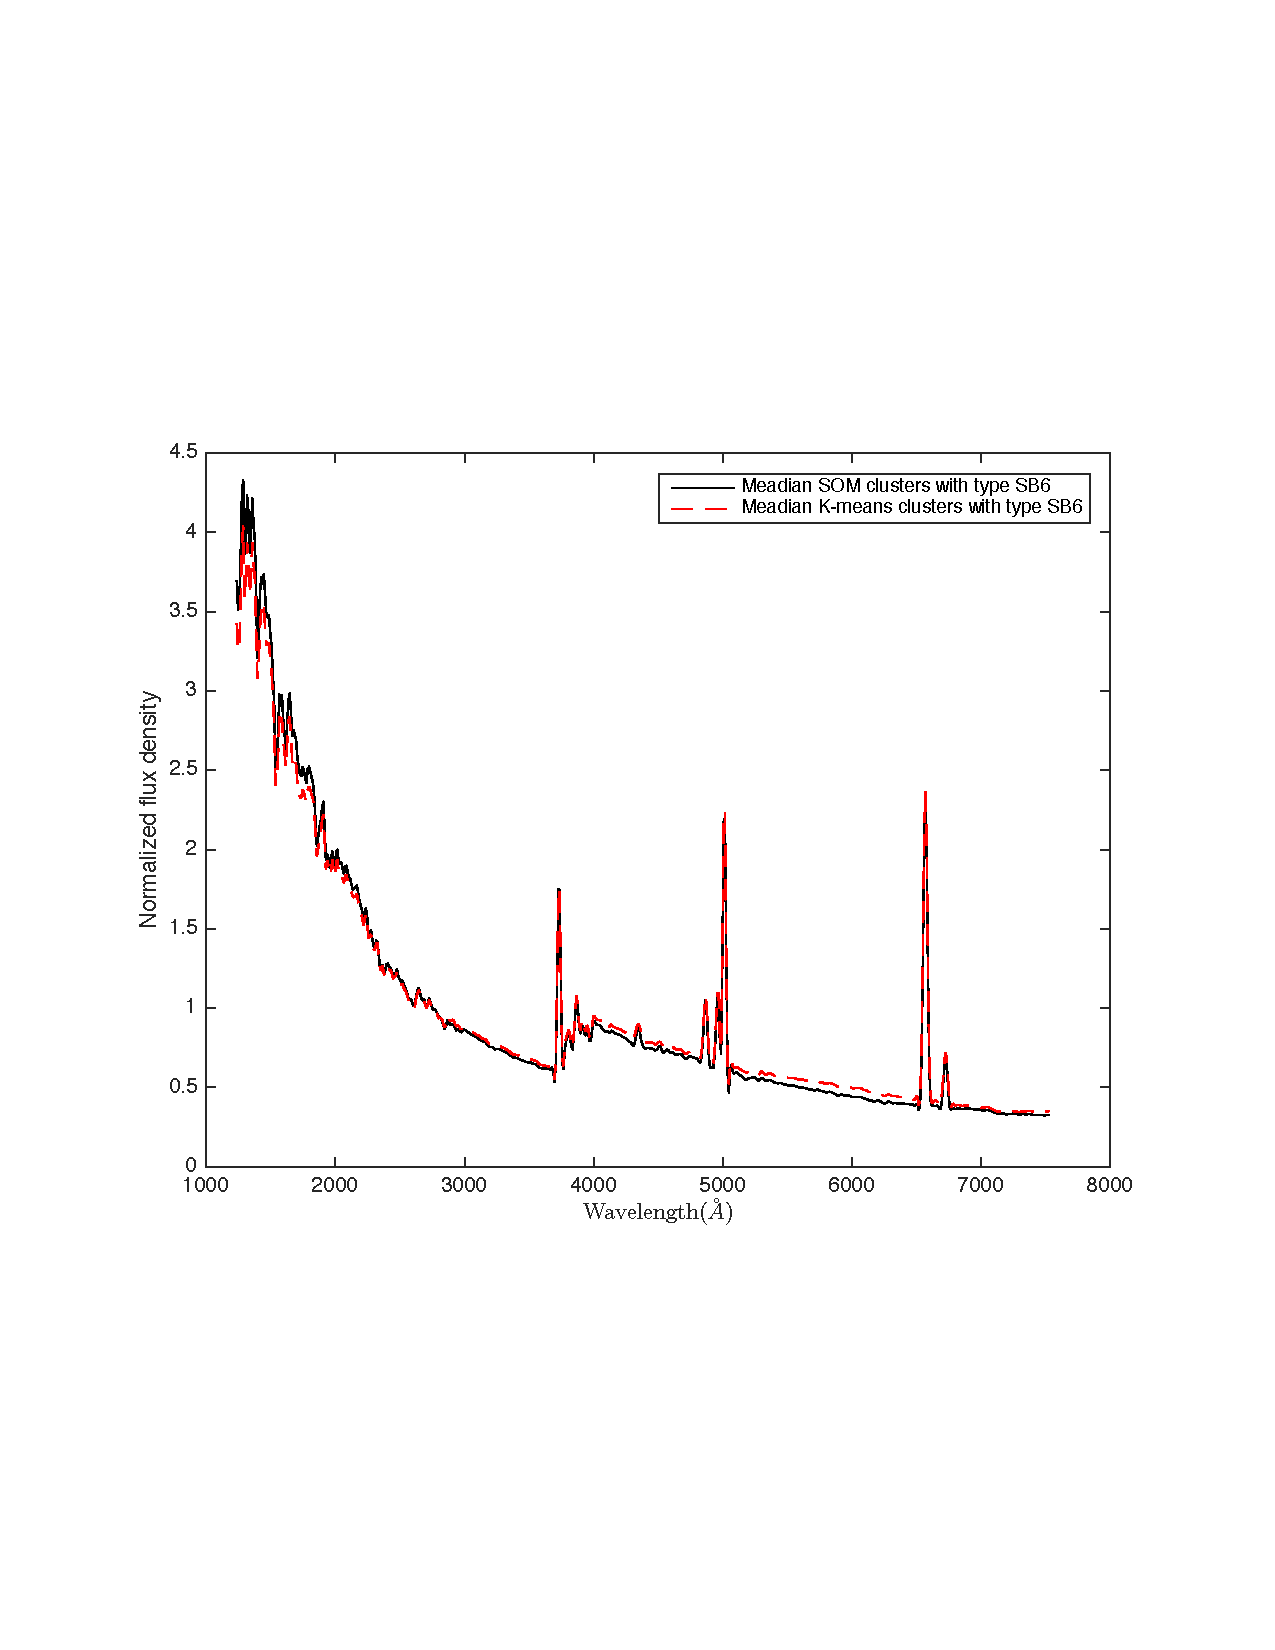
\includegraphics[width=0.99\textwidth]{k_means_images/SB6_comp.pdf}
                \end{subfigure}
                \hfill
                \begin{subfigure}[b]{0.5\textwidth}
                    \centering 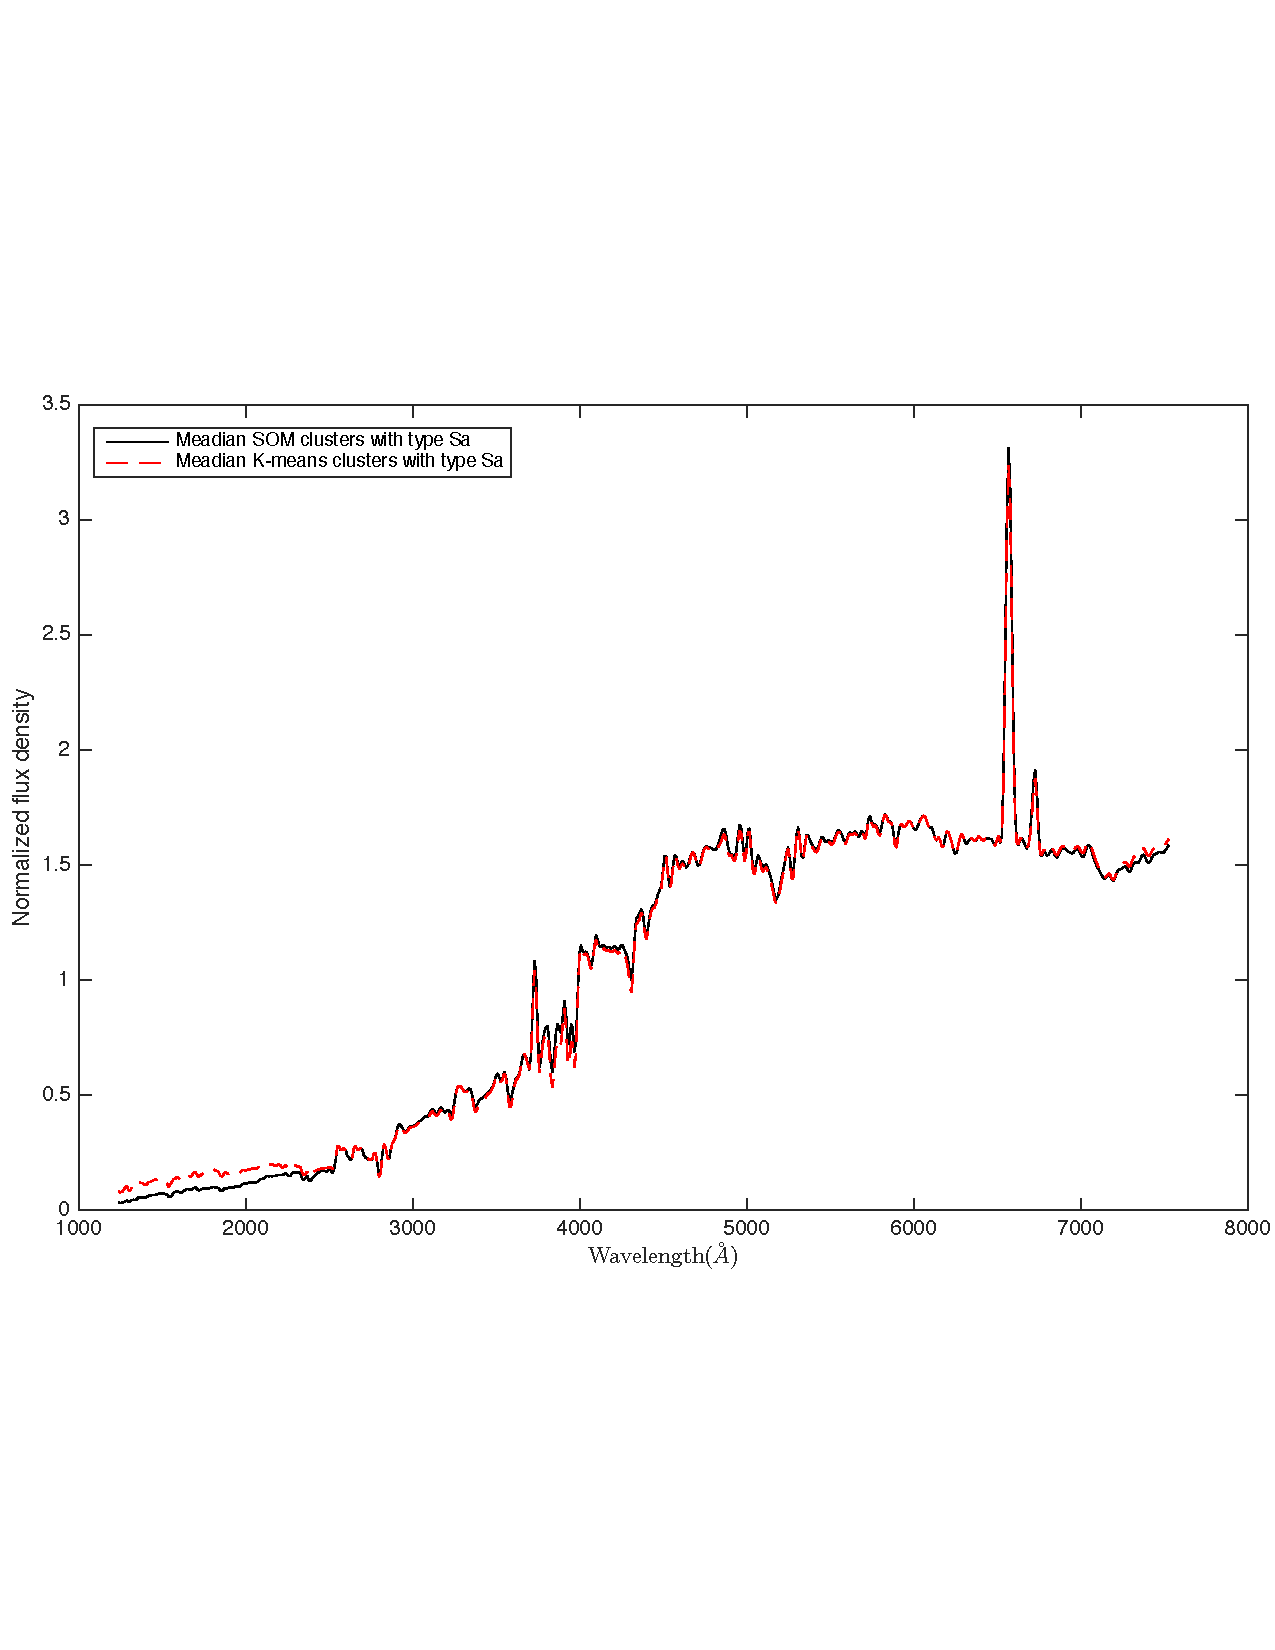
\includegraphics[width=\textwidth]{k_means_images/Sa_comp.pdf}
                \end{subfigure}
                \caption{km}
                 \label{fig: som_k_means_comp}
\end{figure}
